%%% Hlavní soubor. Zde se definují základní parametry a odkazuje se na ostatní části. %%%

%% Verze pro jednostranný tisk:
% Okraje: levý 40mm, pravý 25mm, horní a dolní 25mm
% (ale pozor, LaTeX si sám přidává 1in)
\documentclass[12pt,a4paper]{report}
\setlength\textwidth{145mm}
\setlength\textheight{247mm}
\setlength\oddsidemargin{15mm}
\setlength\evensidemargin{15mm}
\setlength\topmargin{0mm}
\setlength\headsep{0mm}
\setlength\headheight{0mm}
% \openright zařídí, aby následující text začínal na pravé straně knihy
\let\openright=\clearpage

%% Pokud tiskneme oboustranně:
% \documentclass[12pt,a4paper,twoside,openright]{report}
% \setlength\textwidth{145mm}
% \setlength\textheight{247mm}
% \setlength\oddsidemargin{15mm}
% \setlength\evensidemargin{0mm}
% \setlength\topmargin{0mm}
% \setlength\headsep{0mm}
% \setlength\headheight{0mm}
% \let\openright=\cleardoublepage

%% Pokud používáte csLaTeX (doporučeno):
%\usepackage{czech}
%% Pokud nikoliv:
\usepackage[czech]{babel}
\usepackage[T1]{fontenc}

%% Použité kódování znaků: obvykle latin2, cp1250 nebo utf8:
\usepackage[utf8]{inputenc}

%% Ostatní balíčky
\usepackage{graphicx}
\usepackage{amsthm}
\usepackage{amsmath}

%% Balíček hyperref, kterým jdou vyrábět klikací odkazy v PDF,
%% ale hlavně ho používáme k uložení metadat do PDF (včetně obsahu).
%% POZOR, nezapomeňte vyplnit jméno práce a autora.
\usepackage[unicode]{hyperref}   % Musí být za všemi ostatními balíčky
\hypersetup{pdftitle=Hledání pěších cest v~mapě}
\hypersetup{pdfauthor=Tomáš Pokorný}

%%% Drobné úpravy stylu

% Tato makra přesvědčují mírně ošklivým trikem LaTeX, aby hlavičky kapitol
% sázel příčetněji a nevynechával nad nimi spoustu místa. Směle ignorujte.
\makeatletter
\def\@makechapterhead#1{
  {\parindent \z@ \raggedright \normalfont
   \Huge\bfseries \thechapter. #1
   \par\nobreak
   \vskip 20\p@
}}
\def\@makeschapterhead#1{
  {\parindent \z@ \raggedright \normalfont
   \Huge\bfseries #1
   \par\nobreak
   \vskip 20\p@
}}
\makeatother

% Toto makro definuje kapitolu, která není očíslovaná, ale je uvedena v obsahu.
\def\chapwithtoc#1{
\chapter*{#1}
\addcontentsline{toc}{chapter}{#1}
}

\begin{document}

% Trochu volnější nastavení dělení slov, než je default.
\lefthyphenmin=2
\righthyphenmin=2

%%% Titulní strana práce

\pagestyle{empty}
\begin{center}

\large

Univerzita Karlova v~Praze

\medskip

Matematicko-fyzikální fakulta

\vfill

{\bf\Large BAKALÁŘSKÁ PRÁCE}

\vfill

\centerline{\mbox{
\includegraphics[width=60mm]{../img/logo.eps}}}

\vfill
\vspace{5mm}

{\LARGE Tomáš Pokorný}

\vspace{15mm}

% Název práce přesně podle zadání
{\LARGE\bfseries Hledání pěších cest v~mapě}

\vfill

% Název katedry nebo ústavu, kde byla práce oficiálně zadána
% (dle Organizační struktury MFF UK)
Katedra aplikované matematiky

\vfill

\begin{tabular}{rl}

Vedoucí bakalářské práce: & Mgr. Martin Mareš, Ph.D. \\
\noalign{\vspace{2mm}}
Studijní program: & Informatika \\
\noalign{\vspace{2mm}}
Studijní obor: & Obecná informatika \\
\end{tabular}

\vfill

% Zde doplňte rok
Praha 2014

\end{center}

\newpage

%%% Následuje vevázaný list -- kopie podepsaného "Zadání bakalářské práce".
%%% Toto zadání NENÍ součástí elektronické verze práce, nescanovat.

%%% Na tomto místě mohou být napsána případná poděkování (vedoucímu práce,
%%% konzultantovi, tomu, kdo zapůjčil software, literaturu apod.)

\openright

\noindent
\chapter*{Poděkování}
Na tomto místě bych rád poděkoval Mgr. Martinu Marešovi, Ph.D. za cenné rady a
odbornou pomoc při konzultacích k~této práci. Dále bych rád poděkoval Mgr.
Tomáši Gavenčiakovi za pomoc při ladění aplikace a české komunitě OpenStreetMap
za vysvětlení nejasností ohledně mapových dat.

\newpage

%%% Strana s čestným prohlášením k bakalářské práci

\vglue 0pt plus 1fill

\noindent
Prohlašuji, že jsem tuto bakalářskou práci vypracoval samostatně a výhradně
s~použitím citovaných pramenů, literatury a dalších odborných zdrojů.

\medskip\noindent
Beru na~vědomí, že se na moji práci vztahují práva a povinnosti vyplývající
ze zákona č. 121/2000 Sb., autorského zákona v~platném znění, zejména skutečnost,
že Univerzita Karlova v~Praze má právo na~uzavření licenční smlouvy o~užití této
práce jako školního díla podle §60 odst. 1 autorského zákona.

\vspace{10mm}

\hbox{\hbox to 0.5\hsize{%
V~........ dne ............
\hss}\hbox to 0.5\hsize{%
Podpis autora
\hss}}

\vspace{20mm}
\newpage

%%% Povinná informační strana bakalářské práce

\vbox to 0.5\vsize{
\setlength\parindent{0mm}
\setlength\parskip{5mm}

Název práce:  	
Hledání pěších cest v~mapě
% přesně dle zadání

Autor:
Tomáš Pokorný

Katedra:  % Případně Ústav:
Katedra aplikované matematiky
% dle Organizační struktury MFF UK

Vedoucí bakalářské práce:
Mgr. Martin Mareš, Ph.D., KAM
% dle Organizační struktury MFF UK, případně plný název pracoviště mimo MFF UK

Abstrakt:
Cestování pěšky po městě je součástí každodenního života mnoha lidí. Najít
vhodnou cestu nemusí být ve městě jednoduché. Snažili jsme se vytvořit z dat
projektu OpenStreetMap datové struktury vhodné pro vyhledávání pěších tras ve
městě, včetně možnosti chůze mimo cesty v průchozích oblastech (parky, náměstí). 
Součástí práce je i řešení některých druhů chyb ve vstupních datech. Vytvořili
jsme také aplikaci umožňující trasy hledat a exportovat do formátu GPX.


% abstrakt v rozsahu 80-200 slov; nejedná se však o opis zadání bakalářské práce

Klíčová slova:
mapa, pěší vzdálenosti, hledání trasy
% 3 až 5 klíčových slov

\vss}\nobreak\vbox to 0.49\vsize{
\setlength\parindent{0mm}
\setlength\parskip{5mm}


Title:
Finding footpaths in a map
% přesný překlad názvu práce v angličtině

Author:
Tomáš Pokorný

Department:
Department of Applied Mathematics
% dle Organizační struktury MFF UK v angličtině

Supervisor:
Mgr. Martin Mareš, Ph.D., Department of Applied Mathematics
% dle Organizační struktury MFF UK, případně plný název pracoviště
% mimo MFF UK v angličtině

Abstract:
Walking in the city is a part of everyday life for many people. Finding the right
way is not very easy. From the data of OpenStreetMap project we made data
structures suitable for finding paths for pedesterians, including direct walking through
areas (parks, squares). Fixing some bugs in input data is also a part of the
thesis. We have made an application for finding pedesterian ways and their export
to GPX as well.

% abstrakt v rozsahu 80-200 slov v angličtině; nejedná se však o překlad
% zadání bakalářské práce

Keywords:
map, walking distance, finding paths
% 3 až 5 klíčových slov v angličtině

\vss}

\newcommand{\tuc}{\bf}
\newcommand{\footurl}[1]{\footnote{\url{#1}}}

\newpage

%%% Strana s automaticky generovaným obsahem bakalářské práce. U matematických
%%% prací je přípustné, aby seznam tabulek a zkratek, existují-li, byl umístěn
%%% na začátku práce, místo na jejím konci.

\openright
\pagestyle{plain}
\setcounter{page}{1}
\tableofcontents

%%% Jednotlivé kapitoly práce jsou pro přehlednost uloženy v samostatných souborech
\chapwithtoc{Úvod}

chceme hledat cestu
chceme chodit pěšky
existují různé služby
většina určena primárně pro auta -> nereflektuje pěší potřeby
 - kros průchozích prostranství


Hledání cesty ve městě je častou situací většiny lidí. Ve městě se vyskytuje
mnoho různých překážek jako jsou ploty, zábradlí či frekventované silnice,
i mnoho průchozích prostranství, například náměstí, parky či sady. V naší práci
se snažíme z mapových dat vytvořit formát vhodný pro rychlé vyhledávání pěších
tras využívajících i průchozí prostranství. Tato práce by měla být jedním z~modulů
budoucí aplikace pro vyhledávání spojení pěšky a MHD po městě. 

%\section{Co chci počítat}
Abychom mohli rychle vyhledávat pěší trasy, potřebujeme k~tomu mít mapu vhodně
reprezentovanou. Vstupní mapová data postupně zpracováváme a vybíráme z nich
použitelné informace. Na konci tohoto procesu vytvoříme graf popisující možné
pěší trasy. V tomto grafu již můžeme vyhledávat pomocí grafových algoritmů pro
hledání cest, v ukázkové aplikaci využíváme Dijkstrův algoritmus. 

%\section{Zdroje dat}
Abychom mohli vyhledávat trasy, potřebujeme k~tomu vhodné mapové podklady.
Protože jsme chtěli, aby bylo možné zpracovaná data volně používat a šířit, 
potřebovali jsme získat i takové mapové podklady. Proto jsme si vybrali jako
zdroj dat OpenStreetMap (OSM), volně dostupné mapové podklady vytvářené komunitou. 
Projekt OpenStreetMap využívá k~tvorbě mapy mimo práce dobrovolníků také jiné
volně dostupné mapové podklady a poskytuje pravěpodobně nejlepší veřejně
dostupná mapová data. Jako zdroj dat o~nadmořské výšce jsme použili data
z~projektu SRTM, která jsou také volně dostupná.

%\section{Co už kdo napsal}
K~porovnání výsledků naší aplikace jsme použili nejznámější webové mapové
aplikace -- Google Maps a Mapy.cz. Také jsme nalezené trasy porovnávali s~jinými
vyhledávači používajícími data OSM -- OsmAnd a TODO. Nalezené trasy jsme také
porovnávali s~vlastní znalostí terénu a skutečně používaných cest.

%TODO: obrazek - vstupni data a vystupni data

V první kapitole se zabýváme zdrojovými geografickými daty. Popíšeme, jakým
způsobem OpenStreetMap popisuje objekty reálného světa a jaké to přináší
problémy při zpracování. Ukážeme jeden ze způsobů, kterým jsou data ukládána -
OSM XML. Popíšeme, které informace z dat OSM využíváme a s jakými problémy jsme
se při jejich zpracování museli vypořádat. Na konci se zmíníme o používaných
výškových datech z projektu SRTM.

Ve druhé kapitole popíšeme používané formáty. Popíšeme souřadný systém UTM a
důvody, proč jsme ho zvolili jako interní reprezentaci souřadnic. Popíšeme
ProtocolBuffery používané jako binární reprezentace našich datových struktur.
Popíšeme datovou strukturu používanou při zpracovávání mapových dat a strukturu
vyhledávacího grafu z dat vzniklého.

Ve třetí kapitole popíšeme použité algoritmy

Ve čtvrté kapitole poíšeme detaily implementace jednotlivých fází zpracování,
popíšeme problémy, které při implmentaci nastaly a jakým způsobem jsme je
řešili. 

V páté kapitule se budeme zabývat hledáním ve vygenerovaných datech. Popíšeme
Dijkstrův algoritmus pro vyhledávání v grafu a popíšeme ukázkovou vyhledávací
aplikaci. 

V šesté kapitole porovnáme výsledky naší aplikace s výsledky jiných vyhledávačů
a vlastními zkušenostmi. 



\chapter{Intro}

\section{Cíl práce}
Hledání pěších tras v~terénu je velmi rozsáhlé téma s~mnoha specifickými
podoblastmi. Naším hlavním záměrem je hledání tras ve městě,
protože města jsou dostatečně dobře zmapovaná a zároveň pěší trasy z~různých
současných vyhledávačů nebývají optimální. Navíc máme v~plánu práci dále
rozšiřovat a vytvořit vyhledávač spojení po městě využívající kombinaci pěších
tras a městské hromadné dopravy.  Cílem práce je specifikace vhodného formátu
dat pro vyhledávání pěších tras ve městě a algoritmů pro přípravu mapových dat
do tohoto formátu. 

Nechtěli jsme vytvořit data pro obecný vyhledávač tras, zaměřili jsme se
pouze na pěší trasy a jejich specifika. Také jsme se nesnažili vytvořit komplexní
vyhledávací aplikaci; vyhledávací aplikace je pouze ukázkou, že jsou námi
vytvářená data přímo použitelná pro vyhledávání dosahující dobrých výsledků.

\section{Zdroje dat}
Chtěli jsme, aby bylo možné aplikaci i data volně šířit, proto jsme hledali
zdroj mapových dat, který umožňuje jejich volné užití. Nejznámějším projektem,
který mapová data shromažďuje, je projekt OpenStreetMap. Tento projekt vytváří
mapu světa za pomoci dobrovolníků a také importuje jiná volně dostupná data.
Jedná se o~nejkvalitnější volně dostupná mapová data pro celý svět, proto jsme
tento projekt zvolili jako zdroj mapových dat.

Pro kvalitní hledání potřebujeme i výšková data. Ta používáme z~projektu SRTM,
\cite{srtmweb} protože jsou také volně šiřitená a používaná v~mnoha jiných
mapových projektech.

\section{Postup práce}
Problém hledání trasy v~mapě jsme chtěli převést na problém hledání cesty
v~ohodnoceném grafu. Snažili jsme se proto mapová data postupně zpracovat a
vytvořit z~nich graf s~ohodnocenými hranami, ve kterém pak můžeme snadno
vyhledávat například Dijkstrovým algoritmem. Ohodnocení hran však není v~grafu
uvedeno přímo, hrany a vrcholy obsahují informace, ze kterých ohodnocení
vypočítává až při vyhledávání. Toto ohodnocení může být ovlivňováno nastavením
vyhledávače.

Při přípravě dat nejprve vybereme rozdělíme mapová data do kategorií a společně
s~výškovými daty je uložíme do formátu pro přípravu dat. Data dále zpracováváme,
převedeme složité objekty na jednodušší, budovy v~blocích nahradíme jejich
obvody, příliš dlouhé úsečky rozdělíme na kratší. V~další fázi mezi blízké cesty
přidáme spojovací hrany, což nám pomůže vypořádat se s~problémem nespojených
cest. Poté přidáme zkratky přes průchozí prostranství a nakonec přípravný formát
převedeme na vyhledávací graf. V~tomto grafu pak vyhledáváme Dijkstrovým
algoritmem.

%%\section{Co už kdo napsal}
%K~porovnání výsledků naší aplikace jsme použili nejznámější webové mapové
%aplikace -- Google Maps a Mapy.cz. Také jsme nalezené trasy porovnávali s~jinými
%vyhledávači používajícími data OSM -- OsmAnd a TODO. Nalezené trasy jsme také
%porovnávali s~vlastní znalostí terénu a skutečně používaných cest.
%

\section{Implementační prostředky}
Pro implementaci algoritmů v~naší práci jsme zvolili jazyky Python a C. První část
aplikace připravující z~mapy data pro vyhledávání jsme napsali v~Pythonu. Tento
objektový skriptovací jazyk jsme zvolili z~důvodu předchozích zkušeností a
rychlé tvorby kódu. Jazyk již v~základu poskytuje pokročilé datové struktury a
má širokou databázi knihoven usnadňujících vývoj. 

První implementace druhé části přípravné aplikace používaly také Python, ale programy
běžely příliš pomalu a byly velmi náročné na paměť. Proto jsme se rozhodli na
druhou část použít jazyk C, který má minimální paměťovou režii a je také velmi
rychlý. Jako doplnění tohoto jazyka jsme užili knihovnu LibUCW, která poskytuje
rychlé implementace složitějších datových struktur (stromy, haldy) a algoritmů
(třídění). 

Pro implementaci aplikace pro vyhledávání trasy jsme také zvolili jazyk C pro
paměťovou nenáročnost a rychlost. Při implementaci jsme se snažili využívat
minimum externích knihoven, aby byla aplikace snadno přenostitelná na jiné
platformy. Grafická nadstavba je napsána v~C{\tt++} v~prostředí Qt, protože toto
prostředí umožňuje snadné vytvoření grafického rozhraní a již pro něj existují
komponenty pro zobrazování mapy. Samotná grafická nadstavba pak používá fukce
z~vyhledávače v~C.

%%TODO: obrazek - vstupni data a vystupni data


\chapter{Projekt OpenStreetMap}
\section{O projektu}
Projekt OpenStreetMap\cite{osmweb} vznikl v Anglii v roce 2004 a jeho prvotním cílem bylo
vytvořit volně dostupná geografická data pro Velkou Británii. Iniciativa se
postupně rozrostla do celého světa a dnes mapu pomáhá tvořit přes milion
dobrovolníků. Česká republika je dnes poměrně kvalitně pokryta a zvláště velká
města mají dostatečně detailní pokrytí i pro vyhledávání pěších tras.

\section{Datová primitiva} 
Projekt OpenStreetMap používá tři základní geografická primitiva: uzly, cesty a
relace. Ke každému z těchto primitiv mohou být přiřazeny atributy, což jsou
dvojice klíče a hodnoty. 
U polohových dat se neukládá výška, výsledná mapa je pouze dvourozměrná.
Každé primitivum má jedinečné id.
Nyní popíšeme jednotlivá primitiva

{\tuc Uzly} jsou body s určenými souřadnicemi. Uzly mohou mít atributy, ty pak
určují bodový mapový objekt, například rozcestník nebo závora. Existují i uzly
bez atributů sloužící pouze jako součást cest nebo relací.

{\tuc Cesty} jsou posloupnosti uzlů. Uzly se na cestě nemohou opakovat s
jedinnou výjimkou, že první a poslední bod mohou být shodné, potom se jedná o
uzavřenou cestu. Cesty jsou orientované, tzn. na pořadí uzlů záleží. Mohou
existovat cesty bez atributů jako součásti relace, ale obvykle mají atributy
učující, jaký objekt je jimi reprezentován.

Cestami jsou reprezentovány linie a plochy. Pokud má být cesta plochou, musí být
uzavřená, ale ne každá uzavřená cesta je plocha. Tento problém rozebíráme níže.
Jedna cesta také může reprezentovat více fyzických objektů (například silnici s
tramvajovou tratí, park s oplocením).

{\tuc Relace} jsou posloupnosti uzlů a cest opatřená atributy. Každý prvek v
relaci navíc může mít určenou roli. Relace může obsahovat jako prvek i relaci,
ale tato situace není příliš dobře podporována.  Obvykle jsou relacemi
reprezentovány složitější objekty, které by se cestami a uzly reprezentovaly
obtížně, jako například trasy linek MHD, cyklotrasy a územní hranice.

Pro nás důležitý typ relace je multipolygon, který se používá k reprezentaci
složitějších ploch. Multipolygon obsahuje cesty s rolemi \verb|INNER| resp.
\verb|OUTER| reprezentující vnitřní respektive vnější okraj plochy.

\section{OSM XML}
Nejobvyklejší způsob ukládání OSM dat je ve formátu XML. Všechna primitiva mají
jako jeden z atributů \verb|id|, který značí jejich jednoznačný identifikátor.
Každý typ primitiva má svou vlastní číselnou řadu. V OSM XML\cite{osmxml} je
nejprve hlavička, následně seznam uzlů, seznam cest a seznam relací. Níže je
příklad takového souboru.

% Pozor na zlom stránky
\begin{verbatim}
<!-- Hlavicka !-->
<?xml version='1.0' encoding='UTF-8'?>
<osm version="0.6" generator="osmconvert 0.7T">
	<bounds minlat="49.4645" minlon="14.334" maxlat="49.466" 
	maxlon="14.339"/>

<!-- Uzly !-->
	<node id="962931066" lat="49.4647188" lon="14.3384903" version="1" 
	timestamp="2010-10-24T05:47:30Z" changeset="6153364" uid="1066" />

<!-- Cesty !-->
	<way id="82704082" version="1" timestamp="2010-10-24T06:27:17Z" 
	changeset="6153364" uid="1066" user="pavel">
		<nd ref="962425008"/>
		<nd ref="962931066"/>
		<nd ref="962738699"/>
		<nd ref="962425008"/>
		<tag k="dibavod:id" v="9890"/>
		<tag k="natural" v="wetland"/>
		<tag k="source" v="dibavod A06"/>
	</way>

<!-- Relace !-->
	<relation id="25793" version="3" timestamp="2012-07-31T09:21:12Z" 
			changeset="12558592" uid="82083" user="petr_balicek">
		<member type="way" ref="26082949" role="outer"/>
		<member type="way" ref="26080423" role="inner"/>
		<member type="way" ref="26080424" role="inner"/>
		<tag k="landuse" v="forest"/>
		<tag k="type" v="multipolygon"/>
	</relation>
	<relation id="2331090" version="3" timestamp="2012-10-03T21:29:24Z"
			changeset="13353948" uid="8007" user="vrabcak">
		<member type="way" ref="174291392" role=""/>
		<tag k="boundary" v="protected_area"/>
		<tag k="leisure" v="nature_reserve"/>
		<tag k="name" v="PP Boukal"/>
		<tag k="type" v="boundary"/>
	</relation>
</osm>
\end{verbatim}

Popišme si nyní jednotlivé části:

{\tuc Hlavička souboru.} V XML hlavičce je určeno kódování UTF-8 a následně je
otevřen element \verb|osm|, jehož atributem je také použitá verze API. 

{\tuc Uzly.} Zde jsou za sebou postupně vypsány všechny uzly. Uzly jsou
reprezentovány elementem \verb|node|, každý má atribut \verb|lat| a \verb|lon|
určující jejich zeměpisnou šířku a délku, používá se souřadný systém
WGS-84\cite{wgsnorma}. Dále mohou
mít vnořené elementy \verb|tag|. Každý tento element má atribut \verb|k|
reprezentující klíč a \verb|v| reprezentující hodnotu pro atributy uzlu.

{\tuc Cesty.} Zde jsou za sebou vypsány cesty. Cesty jsou reprezentovány
elementem \verb|way|, v němž jsou vnořeny elementy \verb|nd|. Každý element
\verb|nd| reprezentuje jeden uzel na cestě, identifikátor tohoto uzlu je uložen
v atributu \verb|ref|. Také cesty mohou mít vnořené elementy \verb|tag|.

{\tuc Relace.} Jako poslední jsou vypsány všechny relace, reprezentované
elementem \verb|relation|. Prvky relací jsou reprezentovány elementy
\verb|member|, které obsahují atributy \verb|type| určující, o jaký typ
primitiva jde, \verb|ref| určující identifikátor tohoto primitiva a \verb|role|
určující roli daného prvku v relaci. I relace mohou mít vnořené elementy
\verb|tag|.


Toto pořadí umožňuje proudově zpracovávat XML, protože když zpracováváme cesty,
tak již máme v paměti všechny uzly, na které se cesty mohou odkazovat, obdobně
s relacemi. 

OSM XML se dá volně stáhnout, většinou jsou tyto soubory pro úsporu místa
zaarchivované a aktualizují se jednou denně. Protože většina aplikací
nepotřebuje data z celého světa, jsou k dispozici i data pro jednotlivé
kontinenty a státy\footnote{\url{http://osm.kyblsoft.cz/archiv/}}. 

\section{Problémy v datech}
Ačkoli jsou data z OSM poměrně kvalitní a přesné, během jejich zpracování jsme
narazili na některá problematická místa. 

{\tuc Různorodé označování ploch.} Tento problém plyne již z definice geografických
primitiv a atributů objektů. Protože jak plochy, tak linie jsou označovány v OSM
stejným primitivem {\em cesta}, musí se při rozlišování hledět na jejich atributy.
Bohužel ani zde není jejich používání sjednoceno. Aby mohla být {\em cesta}
plochou, musí mít první a poslední {\em uzel} stejný. Ale ne každá uzavřená {\em
cesta } je plochou. Například uzavřená silnice se pokládá za kruhový objezd a
nikoli plochu. Aby byla považována za plochu, musí mít nastaven klíč
\verb|area| hodnotu \verb|yes|. Naopak pokud má {\em cesta} například klíč \verb|landuse|
nebo \verb|building|, je za plochu považována, i když nemá klíč \verb|area|.

{\tuc Nekorektní objekty.} I přesto, že editory používané pro úpravu OSM se snaží
hlídat správnost vytvořených objektů, se v mapě vyskytují různé chybně
definované objekty. Nalezli jsme například cesty, které samy sebe kříží,
chybějící elementy v hranicích multipolygonu a jiné. Výhodou OSM je, že jsme je
mohli ihned opravit, ale přesto je musí umět program korektně vyhodnotit.

{\tuc Více bodů na stejných souřadnicích.} Ač by se pro spojování sousedních ploch měly
využívat společné body na hranicích, v některých oblastech jsme našli
problematická místa, kde polovina ploch používala jeden bod a druhá polovina
jiný na stejných souřadnicích. Tyto dva body spolu nebyly nijak propojeny a
pravděpodobně vznikly při některém importu z jiných datových zdrojů. Bohužel
takovéto složité chyby se nedají jednoduše ručně opravit a je opět potřeba je
korektně zpracovat.

{\tuc Různá sémantika atributů na různých místech.} Při výběru atributů, které zahrnout
ke zpracování, jsme se setkali s používáním stejných atributů v různých
významech. Například klíč \verb|landuse| s hodnotou \verb|residential| v
některých místech označoval velké plochy s obytnými budovami, jinde volně
přístupná prostranství mezi těmito budovami. Kvůli těmto nejednoznačnostem jsme
některé atributy nemohli použít, protože by vytvářely v některých částech města
nekorektní výsledky.

{\tuc Neúplně navazující cesty.} Kvalita mapovaných cest v OSM je silně závislá na typu
cesty. Zatímco silnice, které jsou často využívány pro hledání tras, jsou
většinou navzájem navázány správně, chodníky často v datech úplně chybí, nebo
nejsou napojeny na silnice. Rovněž přechody často chybí. Proto v našem programu
zkoumáme i okolí cest a přidáváme možné spojky mezi chodníky a silnicemi.

\section{Využívané informace z OSM}
Protože chceme umět nejen vyhledávat po cestách, ale i vytvářet trasy přes
průchozí prostranství, potřebujeme mimo cest zpracovávat i budovy, prostranství 
a další objekty. Zpracováváme cesty, které popisují fyzické objekty v terénu,
naopak vynecháváme správní hranice, podzemní objekty (např. metro) a cesty
popisující služby a občanskou vybavenost. Uzly zpracováváme jen jako body s
danou polohou, jejich atributy nevyužíváme. Z relací používáme pouze
multipolygon, kterým jsou často reprezentovány budovy.


\section{Výšková data}
Abychom mohli správně odhadnout náročnost pěší trasy, musíme znát i informace
o~nadmořské výšce jednotlivých bodů. Stejně tak jako většina jiných projektů jsme
použili data SRTM \cite{srtmweb}, což jsou volně dostupná výšková data pro celý
svět.

Shuttle Radar Topography Mission byl projekt NASA, kdy při letu raketoplánu
Enedavour v roce 2000 byla pomocí radarové interferometrie změřena velká část
Země a zpracovaná data byla následně poskytnuta volně k dispozici.
\footnote{\url{http://dds.cr.usgs.gov/srtm/version2_1/}} 

Výšková data byla měřena po třech úhlových vteřinách (v USA po jedné vteřině),
tudíž v České republice jsou data v mřížce $90\times60$\,m. Data jsou rozdělena
do tabulek po jednom stupni, přičemž sousední tabulky se vždy jedním sloupcem
nebo řádkem překrývají. Každá tabulka má tedy 1201 sloupců a 1201 řádků, kde
řádky odpovídají zeměpisné šířce a sloupce zeměpisné délce.

Nadmořské výšky jsou kódovány celými 16bitovými čísly v big-endian udávajícími
nadmořskou výšku v metrech. Pokud se v některém místě nepodařilo výšku změřit,
je udávána jako -32768. Tabulka je kódována jako binární soubor, kde jsou
jednotlivé řádky zapsány za sebou.

\chapter{Formáty}
Našim cílem je vytvořit data ve formátu vhodném na rychlé vyhledávání pěších
tras. K~tomu potřebujeme jednak samotný formát a jednak postup, kterým z~OSM a
SRTM dat vytvoříme kvalitní data pro vyhledávání. Při výběru vhodného formátu
ukládání dat jsme zvolili Protocol Buffery\cite{pbfweb} vyvinuté Googlem. Data
pro vyhledávání budeme ukládat jako graf, jako seznam vrcholů a seznam hran.



\section{Protocol Buffer}
Protocol Buffer je technologie vyvinutá Googlem a jejím cílem je vytvořit způsob
pro ukládání strukturovaných dat, který by byl jednoduchý, rychlý a nezávislý na
použitém programovacím jazyku a platformě. 

Strukturu dat nejprve popíšeme ve zvláštním souboru pomocí definovaného
jazyka\cite{pbfspec}. Z~něj se následně generují funkce pro použití
v~jednotlivých programovacích jazycích. Základní jednotkou pro přenos dat je
zpráva, která obsahuje datové položky. Každá položka má určenou násobnost, typ a
značku.

\begin{verbatim}

package graph;
import "types.proto";

message Vertex {
    required sint64 idx = 4;
    required sint64 osmid = 1;
    required double lat = 2;
    required double lon = 3;
    optional sint32 height = 5;
    
}

message Graph {
    repeated Vertex vertices = 1;
    repeated Edge edges = 2;
}
\end{verbatim}

{\tuc Násobnost} určuje, kolik prvků může být v~položce uloženo. Možnosti jsou
\verb|required|, pak musí každá zpráva mít v~položce právě jeden prvek,
\verb|optional|, pak ve zprávě tato položka může, ale nemusí mít přiřazen prvek,
\verb|repeated|, pak ve zprávě může být pod položkou uloženo libovolné množství
prvků, i žádný. Tato násobnost fugnuje obdobně jako pole v~programovacích
jazycích. 

{\tuc Typy} jsou podobné typům v~programovacích jazycích, obsahují několik typů celých
čísel, čísla s~plovoucí desetinnou čárkou, řetězce a logické hodnoty. Typem může
být také zpráva, což umožňuje hierarchické strukturování dat. 

{\tuc Jméno} položky slouží pro generování jmen funkcí pro přístup k~dané
položce. Ve vygenerované binární podobě zprávy není obsaženo. 

{\tuc Značka} je jednoznačný číselný identifikátor každé položky, musí být v~rámci
zprávy jedinečná a pokud se formát zprávy v~čase mění, neměly by se značky znovu
používat pro jiné položky.

Dále také může být deklarován výčtový typ, kterým můžeme popisovat prvky
nějaké množiny, je možné vytvářet jmenné prostory pomocí balíčků a používat
definice z~jiných souborů se specifikací.

Když máme specifikovaný formát, necháme si vygenerovat kód pro práci s~tímto
formátem. V~tom je velká výhoda Protocol Bufferů, pomocí kompilátoru se ze
souboru ze specifikací formátu vygeneruje kód v~cílovém jazyce, který nám umožní
pracovat se zprávami jako s~objekty v~objektových jazycích či jako se
strukturami v~C. Takto můžeme s~vytvořenými daty jednoduše pracovat z~mnoha
podporovaných jazyků. Pokud bychom chtěli použít programovací jazyk, který není
podporován, je možné si napsat vlastní dekodér, binární forma Protocol Bufferů
je veřejně zdokumentována.\cite{pbfenc}



\section{Formát pro přípravu dat}
Pro zpracovávání OSM dat jsme navrhnuli vlastní formát, protože formát OSM
obsahuje mnoho údajů, které nepotřebujeme a je tak zbytečně pomalý na zpracování
a naopak některé údaje, které vytváříme během zpracování, by se v~něm obtížně
reprezntovaly. Základní struktura zůstává zachována. Mapu ukládáme jako zprávu
\verb|Map|, která obsahuje seznamy zpráv \verb|Node| pro uzly, \verb|Way| pro
cesty a \verb|Multipolygon| pro multipolygony. Jiné typy relací nejsou
využívány, proto se do tohoto formátu neukládají.

Zpráva \verb|Node| pro uzel obsahuje položky:
\begin{itemize}
	\item \verb|id| -- OSM identifikátor uzlu
	\item \verb|lat| -- zeměpisná šířka v~UTM
	\item \verb|lon| -- zeměpisná délka v~UTM
	\item \verb|height| -- nadmořská výška v~metrech
	%\item \verb|objtype| -- typ uzlu
	\item \verb|inside| -- logická hodnota vyjadřující, zda leží uzel uvnitř
	nějaké překážky, například uzly reprezentující pasáž procházející domem
	%\item \verb|nodeidx| -- pořadí uzlu v seznamu
\end{itemize}
Seznam uzlů se v~průběhu zpracování mění, jsou z~něho mazány uzly, které již
nebudou potřeba a jsou do něj přidávány uzly vzniklé například dělením příliš
dlouhých úseků.

Zpráva \verb|Way| pro cestu obsahuje položky:
\begin{itemize}
	\item \verb|id| -- OSM identifikátor cesty
	\item \verb|refs| -- seznam OSM identifikátorů uzlů, ze kterých se cesta
	skládá
	\item \verb|area| -- logická hodnota určující, jestli je daná cesta
	plochou
	%\item \verb|barrier| -- logická hodnota určující, jestli je daná cesta
	překážkou
	\item \verb|type| -- kategorie reprezentovaného objektu TODO: odkaz
	%\item \verb|bordertype| -- pokud je cesta plocha, jakým způsobem je
	ohraničena
	%\item \verb|crossing| -- jaké kategorie cest cesta kříží
	\item \verb|bridge| -- logická hodnota vyjadřující, zda vede cesta na mostě
	\item \verb|tunnel| -- logická hodnota vyjadřující, zda vede cesta
v~tunelu, průchodu, \dots
	%\item \verb|wayidx| -- pořadí cesty v seznamu
	%\item \verb|render| -- logická hodnota vyjadřující, jestli se bude cesta rednerovat
\end{itemize}
Seznam hran se v~průběhu zpracování také mění, jsou do něj přidávány obrysy
bloků budov a naopak odebírány obrysy jednotlivých budov v~bloku.

Zpráva \verb|Multipolygon| slouží k~uložení těch relací, které jsou
multipolygony. Obsahuje následující položky:
\begin{itemize}
	\item \verb|id| -- OSM identifikátor relace
	\item \verb|refs| -- seznam OSM identifikátorů cest, ze kterých se
	multipolygon skládá
	\item \verb|roles| -- role jednotlivých cest (zda jde o~vnitřní či vnější
	okraj)
	\item \verb|type| -- kategorie reprezentovaného objektu
\end{itemize}
Seznam multipolygonů se v~průběhu zpracování zkracuje, multipolygony jsou
převáděny na cesty a žádné nové vytvářeny nejsou.



\section{Formát vyhledávacího grafu}
Graf ukládáme jako dva seznamy --- seznam vrcholů a seznam hran. U~každého
vrcholu si pamatujeme jeho souřadnice ve formátu UTM, jeho nadmořskou výšku
v~metrech a jeho identifikátor v~OSM. U~hrany si pamatujeme počáteční a koncový
vrchol a její typ značící typ cesty, kterou reprezentuje. Všechny hrany jsou
brány jako obousměrné.

Vyhledávací graf ukládáme jako zprávu \verb|Graph| se dvěma položkami ---
seznamem vrcholů \verb|vertices| a seznamem hran \verb|edges|. Zpráva
\verb|Vertex| popisující vrchol obsahuje položky:
\begin{itemize}
	\item \verb|osmid| -- identifikátor vrcholu v~OSM
	\item \verb|lat| -- zeměpisná šířka v~UTM
	\item \verb|lon| -- zeměpisná délka v~UTM
	\item \verb|height| -- nadmořská výška v~metrech
\end{itemize}
Zpráva \verb|Edge| popisující hranu obsahuje tyto položky:
\begin{itemize}
	\item \verb|vfrom| -- index prvního vrcholu
	\item \verb|vto| -- index druhého vrcholu
	\item \verb|type| -- typ cesty, po které hrana vede
\end{itemize}


\chapter{Příprava dat}
V~této kapitole popíšeme, jak z~OSM dat vyrobíme graf pro vyhledávání pěších
tras. Nejprve z~dat vybereme pouze ta, která potřebujeme, a uložíme je do
našeho formátu k~dalšímu zpracování. Poté zjednodušíme budovy, rozdělíme příliš
dlouhé cesty, doplníme spojky mezi cestami, připravíme zkratky pro trasy přes
průchozí prostranství a nakonec ze všech dat vytvoříme vyhledávací graf.

\section{Klasifikace OSM dat} \label{label:kategorie}
V~našem formátu pro přípravu dat jsou cesty a multipolygony rozděleny do
kategorií podle toho, jaký druh skutečného objekt je jimi reprezentován. Cesty vzniklé
jako zkratky přes průchozí prostranství dostanou kategorii plochy, přes kterou
vedou. Když následně hledáme cestu, můžeme jednotlivým kategoriím přiřadit
rychlosti, jakými se po nich pohybujeme. Kategorie jsou následující:
\begin{itemize}
	\item \verb|WAY| -- cesta, o~které nic nevíme; rezervováno pro speciální
	případy
	\item \verb|WATER| -- strouha či přeskočitelný potok
	\item \verb|PARK| -- plocha s~udržovanou zelení, nízkou trávou
	\item \verb|GREEN| -- plocha s~neudržovanou zelení, často jsou v~ní
	prošlapané nezmapované cestičky
	\item \verb|FOREST| -- les v~městském slova smyslu, obvykle bývá pěšky
	průchozí
	\item \verb|PAVED| -- zpevněná cesta či plocha
	\item \verb|UNPAVED| -- nezpevněná cesta či plocha
	\item \verb|STEPS| -- schody
	\item \verb|HIGHWAY| -- silnice, silnice s~chodníkem
	\item \verb|BARRIER| -- překážka pro chodce nepřekonatelná, typ se
	nerozlišuje, například budova, řeka, plot, dálnice
	\item \verb|DIRECT| -- spojka mezi cestami -- krátké cesty generované
	pro doplnění chybějících napojení chodníků na silnice apod.
\end{itemize}
Rozdělení do kategorií probíhá s~pomocí konfiguračního souboru, ve kterém můžeme
zvolit jaké atributy mají objekty mít, aby patřily do dané kategorie. Protože
ani informace, zda jde o~plochu, není ve specifikaci OSM přesně definována, jsou
pro určení, zda jde o~plochu, použity údaje z~konfiguračního souboru. Po
rozdělení objektů do kategorií jsou smazány body, které neleží na žádné cestě,
protože takovéto body dále nikde nepotřebujeme.

\section{Převod multipolygonů na obvodové cesty}
Protože plochy popisované pomocí multipolygonů mají složitou strukturu a obtížně
by se nám s nimi pracovalo, nahradíme multipolygony cestami reprezentujícími
vnější obvody jednotlivých komponent multipolygonů.

Abychom vytvořili obvody jednotlivých komponent, potřebujeme vědět, které cesty
patří do které komponenty.  Dokud nám nějaké cesty zbývají, skládáme z nich
obvody komponent. Cesty na obvodu smažeme a nahradíme jednou uzavřenou cestou
reprezentující celý obvod komponenty. Pokud nemůžeme vytvořit ze zbývajících
cest kružnici -- obvod, pak vypíšeme chybu a multipolygon dále nezpracováváme.
Stejně se zachováme i v případě, že kružnice končí v jiném než počátečním bodě.
Obě tyto situace vznikají kvůli chybám ve zdrojových datech.

\section{Spojení budov}
Ve městě jsou velmi časté bloky budov. V~OSM datech jsou budovy obvykle reprezentovány
samostatně, přičemž nám stačí znát obvod celého bloku. Proto cesty
v~jednotlivých blocích nahradíme jednou cestou reprezentující obvod tohoto bloku.
Nejprve vybereme všechny budovy a vytvoříme si z~nich graf sousednosti
jednotlivých budov. Poté v~každé komponentě najdeme bod na obvodu a postupně
obejdeme po obvodu celou budovu a vytváříme při tom novou cestu. Původní
cesty budov potom smažeme. Když máme zpracované všechny budovy, smažeme body uvnitř
bloku, které nyní neleží na žádné cestě.

Při zpracování se mohou vyskytnout dva druhy problémů. Jednak se uvnitř bloků
mohou vyskytovat cesty, v~tom případě spojování cest přerušíme, protože bychom
se mohli připravit o~možnost přidání spojek mezi cestami uvnitř bloku. Druhý
problém souvisí s~problémem více bodů na stejných souřadnicích. V případě, že
budovy nejsou zcela korektně navázané, vytvoříme z nich korektní cestu, která
ale může obsahovat některé hrany navíc. Budovy také mohou mít na obvodu dva sousední body
na stejných souřadnicích. Pokud narazíme na tuto situaci, zjednodušování
ukončíme, protože nedokážeme určit, jestli tento bod leží na cestě tvořící
obvod, nebo na cestě vedoucí dovnitř budovy. Tento problém se ale nevyskytuje
příliš často, proto jsme ho speciálně neošetřovali.

\section{Rozdělení dlouhých úseků}
Pro další zpracování se nám bude hodit, abychom cesty, po kterých budeme
plánovat trasy, neměly příliš dlouhé úseky. Proto se na všechny takové cesty
podíváme a v~případě, že obsahují úseky delší než zvolená vzdálenost, tyto úseky
rovnoměrně rozdělíme na kratší. 

\section{Spojky mezi cestami}
Jak již bylo zmíněno, chodníky jsou v~OSM zmapovány jen některé a často nejsou
na sebe správně navázány. Proto jsme se rozhodli prohledat okolí každého uzlu a
spojit každé dva uzly, které jsou k~sobě blíže než 20\,m, úsečkou. Při zkoumání
OSM dat jsme zjistili, že mnohé obytné domy kolem sebe nemají značené ploty a
proto jsme vzdálenost zvolili takto nízkou, aby pravděpodobnost, že
jde například o~dvě ulice oddělené domky se zahrádkami, zůstala poměrně malá.  

V oblastech, kde se nacházelo velké množstí uzlů blízko sebe, například u cest
reprezentujících kruhové objezdy, vznikalo příliš velké množství spojek. Tyto
spojky navíc nepřinášely významné zkrácení trasy. U~každého uzlu jsme proto
náhodně vybrali jen některé spojky (viz obr. \ref{fig:spojky}.

\begin{figure}[h]
	\centering
	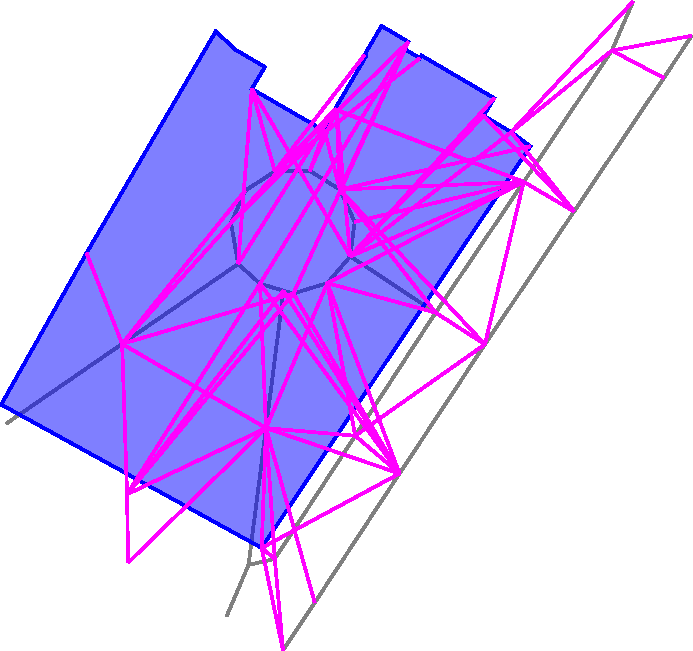
\includegraphics{../img/spojky.pdf}
	\caption{Spojky na malém území. Pokud bychom zde nevybírali náhodně, získali
	bychom velké množství spojek, které by zkrácení trasy příliš nepomohly.
	Růžové úsečky značí vytvořené spojky po náhodném výběru.}
	\label{fig:spojky}
\end{figure}

Spojky navíc mohou vést přes nějakou překážku, jako je plot nebo zeď, proto
potřebujeme zkontrolovat kolize všech přidaných spojek s~překážkami. K~tomuto
účelu jsme využili algoritmus využívající zametání roviny.


{\tuc Zametání roviny} \cite{zametani} je způsob návrhu geometrického algoritmu,
při němž rovinou posouváme přímku (\uv{zametáme}). Pokud přímka protne pro nás
zajímavé místo, vyvoláme událost. Během procházení si obvykle navíc pamatujeme
seznam prošlých bodů nebo aktuálně protnutých úseček, tzv. {\tuc průřez}.

V~našem případě budeme hledat průsečíky úseček v~rovině. Spojky již úsečky jsou,
překážky rozdělíme na jednotlivé úsečky mezi uzly. Budeme zametat podle od
západu k východu a zajímat nás budou události začátku a konce úsečky a jejich
průsečík. Zametací přímku proto budeme posouvat postupně po těchto událostech.

Začátky a konce úseček známe již před spuštěním algoritmu. Průsečíky na začátku
neznáme, budeme ale předpokládat, že se neprotínají tři úsečky v jednom bodě.
Potom platí, že pokud se nějaké dvě úsečky mají protnout, pak se předtím musí
stát sousedními. Proto nám stačí při každé události s úsečkou $u$ stačí
zkontrolovat sousedy $u$ a pokud se s nějakým protíná a průsečík je před
zametací přímkou, přidáme ho do seznamu událostí.

\begin{figure}[h]
	\centering
	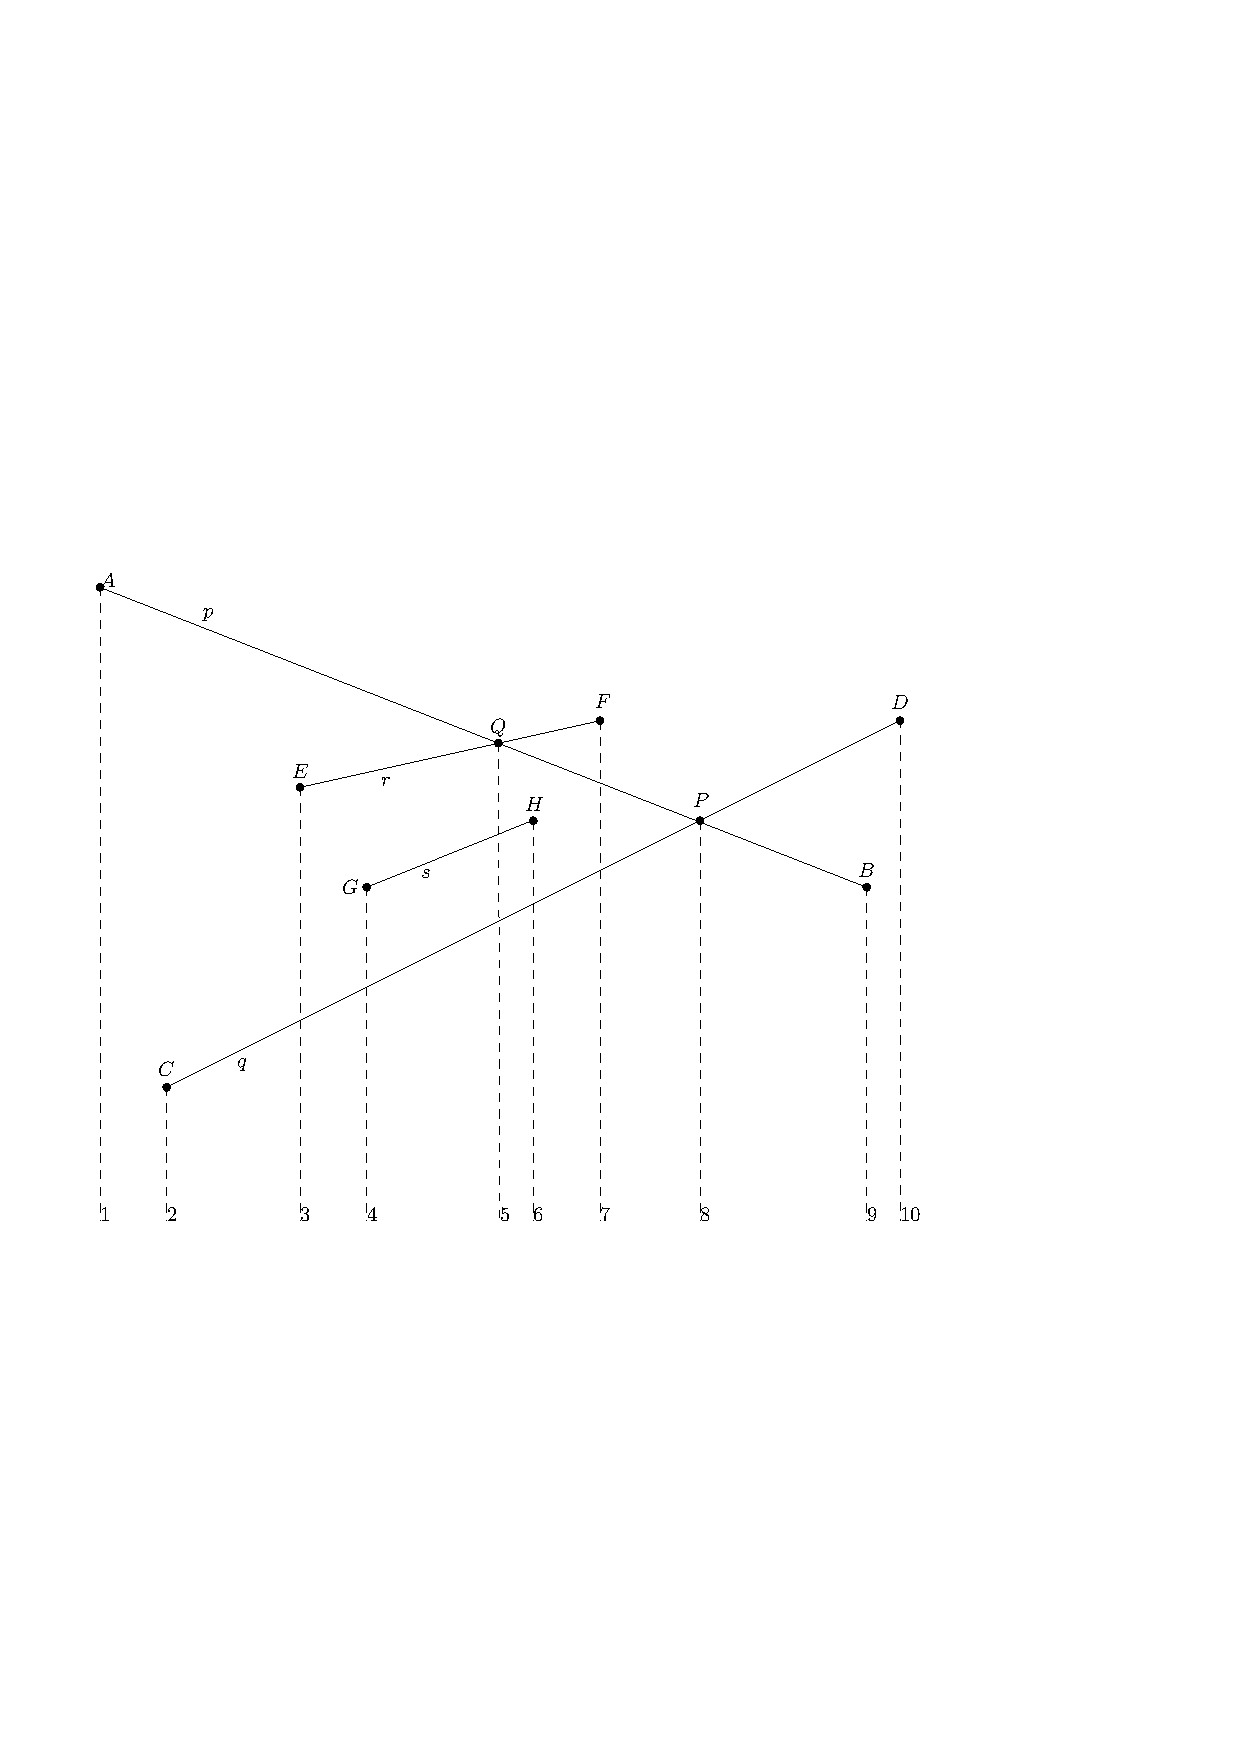
\includegraphics{../img/zametani.pdf}
	\caption{Zametání roviny}
	\label{fig:zametani}
\end{figure}

Protože vždy budeme potřebovat znát nejbližší událost, budeme si udržovat
události v~haldě. Dále také potřebujeme znát pořadí, v~jakém aktuálně
zpracovávané úsečky protínají rovinu -- průřez, a umět mezi ně přidat další a
odebrat tu, která skončí. K~tomuto účelu se nám hodí použít vyhledávací strom.
Nemůžeme si ovšem ve vrcholech pamatovat přímo souřadnice průsečíku úsečky se
zametací přímkou, protože se tyto souřadnice mění s~každým posunutím zametací
přímky. Místo toho si budeme ve stromě pamatovat jen odkazy na úsečky a průsečíky
budeme počítat, až to bude potřeba.

Na začátku známe všechny začátky a konce úseček, vytvoříme tedy v~haldě události
začátků a konců úseček. Průsečíkové události zatím žádné neznáme, ale protože
aby mohl nastat průsečík, musí nejprve úsečka začít, o~žádný nepřijdeme.

Zametání ukázkových dat se čtyřmi úsečkami ukazuje obrázek \ref{fig:zametani}.
Svislé přerušované čáry udávají pozice zametací přímky při vyvolání události,
události nastávají v pořadí 1 až 10.

Zametání bude probíhat následovně. Z~haldy všech událostí vybereme nejbližší
událost a rozhodneme se podle jejího typu:
\begin{itemize}
	\item {\tuc Začátek úsečky.}  Úsečku zařadíme na správné místo do
	průřezu a přidáme případné průsečíkové události se sousedními
	úsečkami.\\
	V situacích 1 a 4 úsečku pouze přidáme, k průsečíkům nedochází.\\
	V situacích 2 a 3 se úsečky protínají, přidáme průsečíkové události
	$P$ a $Q$.

	\item {\tuc Konec úsečky.} Úsečku odebereme z~průřezu a přidáme
	případnou průsečíkovou událost, pokud se úsečky sousední s~právě
	končící protínají.\\
	V situacích 7, 9 a 10 pouze úsečky odebereme z průřezu.\\
	V situaci 6 se po skončení úsečky $s$ stanou úsečky $p$ a $q$ sousedními
	a navíc se protínají, proto přidáme průsečíkovou událost $P$.
	\item {\tuc Průsečík úseček.} Úsečky v~průřezu prohodíme a přidáme
	případné průsečíkové události s~novými sousedy obou prohazovaných 
	úseček. Pokud jsme již průsečík těchto dvou úseček zpracovávali, událost
	zahodíme, protože úsečky se mohou protnout nejvýše jednou a další události
	jsou pouze násobným přidáním téže události (jako zde průsečíku $P$).\\
	V situaci 8 nemají prohozené úsečky žádné nové sousedy.\\
	V situaci 5 se nově stala úsečka $s$ sousedem prohozené přímky $p$, ale
	nemají společný průsečík, událost tedy nepřidáváme.
\end{itemize}
Takto budeme postupovat, dokud jsou v haldě nějaké události. Pokud zpracováváme 
průsečíkovou událost, zkontrolujeme, zda není některá z~úseček překážka a 
případně úsečky označíme, že se protnuly s~překážkou. 


\section{Zkratky přes průchozí prostranství}
Pokud procházíme ve městě přes větší park nebo náměstí, často nemusíme chodit
jen po chodnících, ale můžeme projít přes prostranství přímo. Přímé cesty přes
průchozí prostranství proto také chceme zanést do vyhledávacího grafu. K~jejich
vytvoření jsme využili modifikovaný algoritmus vytváření spojek mezi cestami.
Dvojice bodů v~průchozích prostranstvích jsme spojovali úsečkami. Tentokrát jsme
ale hledali dvojice bližší než 300 m, protože parky mohou být poměrně rozlehlé.
Opět jsme nepoužívali všechny dvojice ale jen některé náhodně vybrané, protože
jinak vznikalo příliš mnoho úseček, které vedly podobně, a proto nepřinášely
významné zlepšení vyhledané trasy. Protože i na průchozích prostranstvích se
vyskytují překážky, opět jsme pomocí zametání roviny odstranili všechny úsečky,
které procházely přes nějakou překážku.

\section{Vytvoření vyhledávacího grafu}
Poté, co jsme připravili data, vytvoříme vyhledávací graf. Protože kolize
přímých cest s~překážkami jsme vyřešili již při jejich vytváření, jsou všechny
cesty korektní. Proto se překážkami již dále nezabýváme a pouze z~cest vytvoříme
vyhledávací graf. Pokud byly v datech přítomny cesty nepřipojené ke zbytku a ani 
přidání spojek a zkratek je nepřipojilo, měl by tento graf více komponent. Tyto
převážně malé komponenty nás nezajímají, protože do nich neumíme najít cestu, a
proto použijeme jen největší komponentu. Uložíme seznam všech uzlů, které jsou
na jejích cestách použity a cesty rozdělíme na jednotlivé hrany grafu mezi dvěma
uzly.  U~hran zachováme údaje o~typu cesty, protože je budeme využívat při
vyhledávání.

\chapter{Implementace}
Pro implementaci programu převádějícího OSM data do formátu vyhledávacího grafu
jsme zvolili v~první části Python, protože pro něj existuje široké množství
knihoven, které nám pomohly při řešení jednotlivých dílčích problémů. Při
vytváření spojek mezi cestami a jejich následné kontrole již ale nedostačoval,
proto jsme tuto a další části implementovali v~jazyce C. Mezi těmito částmi
předáváme data pomocí Protocol Bufferu v~souboru. Vyhledávání je také
implementováno v~jazyce C kvůli rychlosti a paměťové nenáročnosti.

\section{Použité knihovny a pomocné programy}
Během implementace programu pro přípravu dat jsme se snažili použít co nejvíce
již existujících knihoven a programů pro jednotlivé řešené problémy. Všechny
tyto knihovny a programy jsou nutné pro spuštění a používání našeho programu. 

\medskip
\noindent Používáme tyto pomocné programy, údaj v závorce udává licenci:
\begin{itemize}
	\item Výřez s~městem z~dat pro republiku vyrábíme pomocí {\tuc
	Osmconvert} (GNU AGPL).\\
	\url{http://wiki.openstreetmap.org/wiki/Osmconvert}
	\item Pro práci s~Protocol Buffery v~Pythonu využíváme třídy generované
	kompilátorem {\tuc protoc} (BSD New).\\
	\url{http://code.google.com/p/protobuf/}
	\item Pro práci s~Protocol Buffery v~C využíváme funkce a struktury
	generované kompilátorem {\tuc protobuf-c} (BSD 2-Clause).\\
	\url{https://github.com/protobuf-c/protobuf-c}
\end{itemize}

\noindent V~programech napsaných v~Pythonu využíváme následující knihovny:
\begin{itemize}
	\item Na parsování konfiguračních souborů používáme {\tuc PyYAML}
	(MIT).\\
	\url{http://pyyaml.org/wiki/PyYAML}
	\item Na parsování OSM XML používáme {\tuc imposm.parser} (Apache).\\
	\url{http://imposm.org/docs/imposm.parser/latest/}
	\item Souřadnice konvertujeme pomocí {\tuc pyproj} (MIT).\\
	\url{http://code.google.com/p/pyproj/}
	\item Pro hledání komponent grafu využíváme {\tuc networkx} (BSD).\\
	\url{http://networkx.github.io/}
\end{itemize}

\noindent V~programech napsaných v~C využíváme následující knihovny:
\begin{itemize}
	\item Datové struktury, dynamická pole a další funkce zajišťuje
	{\tuc LibUCW} (GNU LGPL).\\
	\url{http://www.ucw.cz/libucw/}
	\item Výpočty se zeměpisnými souřadnicemi provádí {\tuc PROJ.4} (MIT).\\
	\url{http://trac.osgeo.org/proj/}
\end{itemize}

Program osmconvert je již zahrnut ve zdrojovém kódu, ostatní knihovny je
potřeba nainstalovat zvlášť.

\section{Datové struktury}
V~průběhu celé přípravy vyhledávacích dat často využíváme několik struktur,
které nyní popíšeme. Datové struktury využívané jen v~konkrétních případech
popíšeme u~těchto případů.

Při přípravě dat používáme několik {\tuc hešovacích tabulek}. Často potřebujeme
získat uzel respektive cestu s~konkrétním identifikátorem, pro tento účel nám
slouží tabulky \verb|nodesIdx| respektive \verb|waysIdx|. V~Pythonu jsou
reprezentovány typem slovník, v~C využíváme součást knihovny LibUCW
\verb|hashtable|. V~obou případech je klíčem OSM identifikátor objektu a
hodnotou index do pole uzlů resp. cest, kde je daný objekt uložen.

U~každé cesty je v~datech uložen seznam uzlů, přes které prochází. Je ale vhodné
mít i pro každý uzel uložen seznam cest, na nichž leží. Pro tento účel
máme seznam \verb|nodeWays|. Je to seznam seznamů, kdy pod indexem $i$ je seznam
všech identifikátorů cest, které prochází uzlem na pozici $i$ v poli všech uzlů.
V~Pythonu jde o~seznam seznamů, v~C je to rostoucí pole rostoucích polí
z~LibUCW.

Během zpracování hledáme uzly blízké daným uzlům. Abychom pro každé takové
hledání nemuseli procházet všechny uzly, vytvoříme si na začátku {\tuc mřížku}.
Tato mřížka dělí plochu mapy na čtverce $20 \times 20$\,m a v~každém čtverci si
uložíme seznam identifikátorů vrcholů, které v~něm leží. Poté nám při hledání
sousedů bodu stačí zjistit, do kterého čtverce patří, a následně prohledat jen
několik okolních čtverců.

Mřížka je vhodnou strukturou pro rozdělení plochy, protože zástavba ve městě je
poměrně homogenní, tudíž zde nejsou příliš velké volné plochy, kde bychom
zbytečně plýtvali pamětí, ani místa, kde by počet bodů ve čtverci mřížky byl
obtížný na zpracování.

V~Pythonu se jedná o~třídu \verb|Raster|, která při vytvoření vyrobí mřížku
z~mapy. Mřížka je uložena v~atributu \verb|raster|, třída má metodu
\verb|getBox(x,y)|, která pro bod se souřadnicemi $(x,y)$ vrátí tuple se
souřadnicemi buňky, ve které se bod nachází. Mřížka \verb|raster| je seznam
seznamů seznamů.

V~C je mřížka reprezentována strukturou \verb|raster_t|. Samotná mřížka je prvek
\verb|raster| této struktury. V~souboru \verb|raster.h| jsou definovány funkce
pro práci s~mřížkou. Funkce \verb|makeRaster(map_t map)| vyrobí z~mapy mřížku a
vrátí ji. Funkce \verb|getRasterBox(raster_t raster, int64_t x, int64_t y)|
dostane jako paramter mřížku a souřadnice bodu a vrátí pole se dvěma prvky --
souřadnicemi buňky, kde se bod nachází. Mřížka \verb|raster| je reprezentována
polem polí rostoucích polí z~knihovny LibUCW.

\medskip


\section{Stažení dat OSM}
Abychom mohli připravovat data pro vyhledávání, musíme nejprve získat data OSM
pro dané město. O~tuto činnost se stará skript \verb|prepare.sh|, který stáhne
data pro celou Českou republiku a pomocí programu \verb|osmconvert| z~ní vyřízne
obdélník s~městem. Ten uloží jako \verb|praha.osm|\footnote{Program byl
připravován pro vyhledávání tras po Praze, proto soubory obvykle obsahují název
praha.} k~dalšímu zpracování.

\section{Příprava dat SRTM}
Kromě dat OSM potřebujeme i údaje o výškách z projektu SRTM. Protože tato data
se, narozdíl od dat OSM, nebudou aktualizovat, není pro jejich stažení skript,
ale je nutné do složky \verb|osm| nahrát soubory \verb|.hgt|, které pokrývají
obdélník s městem. Pomocí programu \verb|merge-srtm| se \verb|hgt| soubory spojí
do jedné velké tabulky, která je uložena jako \verb|heights.txt|. Její první
řádek obsahuje rozsah pokrývaný SRTM tabulkou a další řádky pak obsahují tabulku
výšek.

\section{Klasifikace dat}
Před dalším zpracováním potřebujeme data OSM převést do formátu pro přípravu dat (premap).
K~tomuto účelu slouží program \verb|parse.py|, který si načte konfigurační soubory
a podle nich rozdělí jednotlivé uzly a cesty do kategorií. Současně také přidá k
uzlům údaje o nadmořské výšce a jejich souřadnice převede do UTM. Následně smaže 
všechny uzly, které neleží na žádné cestě, a uloží data do souboru ve formátu 
formátu premap.

Konfigurační soubory jsou soubory ve formátu YAML \cite{yamlspec}. Používají se následující
konfigurační soubory:
\begin{itemize}
	\item \verb|types.yaml| pro rozdělení cest a multipolygonů do
kategorií 
	\item \verb|area.yaml| pro určení, zda je daný objekt plochou
	\item \verb|tunnel.yaml| pro určení, zda je daný objekt tunelem,
	průchodem či jinou podobnou stavbou
	\item \verb|bridge.yaml| pro určení, zda je daný objekt mostem nebo na
	nějakém mostě leží
\end{itemize}

Konfigurační soubory mají následující formát:
\begin{verbatim}
BARRIER: 
    barrier : "*"
    waterway:
        - river
        - canal
WATER:
    waterway:
        - riverbank
        - stream
\end{verbatim}
Konfigurační soubor se skládá z~několika mapování, u~každého klíč určuje, jaká
kategorie resp. hodnota se přiřadí, hodnotou mapování první úrovně jsou mapování
druhé úrovně, které určují, za jakých podmínek se hodnota přiřadí. Přiřazuje se
vždy, když je splněna alespoň jedna podmínka. 

V~mapování druhé úrovně je klíčem vždy klíč vlastnosti objektu OSM. Hodnota může
být dvou druhů. Buď je to \verb|"*"|, pak stačí, že se shoduje klíč vlastnosti
OSM a na hodnoty se nehledí, nebo je hodnota mapování seznam hodnot objektu OSM.
Pokud má objekt OSM pro daný klíč jednu z~těchto hodnot, je  podmínka splněna. 

V~příkladu rozdělujeme do kategorií \verb|BARRIER| a \verb|WATER|. Pokud má
objekt OSM nějaký atribut s~klíčem \verb|barrier|, je tomuto objektu přiřazena
kategorie \verb|BARRIER| nezávisle na hodnotě tohoto klíče. Obdobně je jako
\verb|BARRIER| označen objekt OSM, který má atribut s~klíčem \verb|waterway| a
hodnotou \verb|river|. Pokud má ale objekt atribut s~klíčem \verb|waterway| a
hodnotou \verb|stream|, je klasifikován jako \verb|WATER|.

Při procházení uzlů jim přiřazujeme ze SRTM výšku a převádíme jejich souřadnice
do UTM. Pomocí metody \verb|calcHeight| spočítáme nadmořskou výšku daného uzlu a
následně jeho souřadnice převedeme do UTM. Navíc {\tuc vynásobíme souřadnice UTM
desíti}, čímž bude jednotkou 10\,cm. Taková přesnost nám stačí a můžeme všechny
výpočty provádět v~celých číslech.

Následně vytvoříme hešovací tabulku \verb|nodeWays| a jejím průchodem zjistíme, které
uzly neleží na žádných cestáchi, a tyto uzly smažeme. Nakonec převedeme data do
formátu premap a uložíme jako soubor \verb|praha-pre.pbf| do složky \verb|data|.

\section{Převod multipolygonů na cesty}
S~multipolygony se v~původní formě pracuje obtížně, protože se jejich obvod
skládá z~neseřazených cest. Pro naše účely se hodí vytvořit cesty reprezentující
obvod multipolygonu. Těchto cest může být více, protože multipolygon se může
skládat z~více komponent. 

Pro každý multipolygon si vytvoříme seznam všech vnějších cest. Pak vytvoříme
seznam sousedů \verb|neighs|, který pro každý uzel na některé z~vnějších cest
obsahuje jeho sousedy na těchto cestách. Ve správném případě by takto měl každý
uzel mít dva sousedy. Pokud tomu tak není, skončíme s~chybou. Poté vybereme
jeden uzel na obvodu a postupujeme po jeho sousedech, dokud se do něj opět
nevrátíme. Použité cesty smažeme ze seznamu všech cest a opakujeme, dokud nějaké
cesty zbývají. Pokud se vrátíme na vytvářenou cestu mimo první vrchol, skončíme
s~chybou.

\section{Spojení budov}
Při spojování bloků budov do jejich obrysu nejprve vytvoříme graf sousednosti
budov. Pro jeho reprezentaci použijeme knihovnu \verb|networkx|. Jednotlivé
budovy budou vrcholy v~grafu, pokud budovy sousední, bude mezi jejich vrcholy
hrana. Graf sousednosti vytváříme funkcí \verb|makeNeighGraph|.

Do grafu nejprve přidáme všechny budovy jako vrcholy. Následně procházíme
všechny uzly a u~každého zkoumáme cesty, které jím prochází. Pokud jde jen
o~budovy, pak mezi první budovou a všemi ostatními vytvoříme v~grafu hrany. Pokud
mezi cestami je i nějaká, která není budovou, pak jsou všechny sousední budovy
označeny za vadné a hrany nepřidáváme.

Když máme graf vytvořen, procházíme ve funkci \verb|mergeComponents| jednotlivé
jeho komponenty a ze všech cest v~komponentě, které nejsou vadné, se pokoušíme
vytvořit cestu. Pokud se to povede, přidáme ji mezi cesty a původní cesty
jednotlivých budov vložíme do seznamu ke smazání. Nakonec funkcí
\verb|removeMerged| smažeme všechny budovy, které jsme nahradili jejich obvodem.

Když vytváříme cestu z~obvodu bloku budov pomocí funkce \verb|mergeWays|,
postupujeme obdobně jako při převodu multipolygonů na cesty. Vytvoříme si seznam
\verb|neighs|, který obsahuje pro každý bod na některé ze spojovaných cest
všechny jeho sousedy. Tentokrát ale může být sousedů více a je potřeba vybrat
toho správného. Setřídíme si tedy uzly podle souřadnic lexikograficky a
nejjižnější z nejzápadnějších vezmeme jako první uzel obvodu.  Protože žádný
západnější ani jižnější bod neexistuje, bude tento uzel zcela jistě na obvodu.
Nyní najdeme druhý uzel na obvodu. Vybereme mezi sousedy prvního uzlu ten, který
svírá s~úsečkou vedoucí z~prvního uzlu na jih nejmenší úhel. Žádný uzel přímo na
jih od prvního není, proto všechny úhly budou nenulové. Uzel pod nejmenším úhlem
bude druhým na obvodu.

Pokud máme první dva body na obvodu, stačí nám již jen ze sousedů aktuálně
zpracovávaného uzlu vybrat ten uzel, který svírá s~předchozím a aktuálním uzlem
nejmenší vnější úhel a takto pokračovat, dokud se nevrátíme do prvního uzlu.

Jestliže počet uzlů je menší než tři, nejde o~korektní plochu a je vrácena chyba.
Rovněž pokud během průchodu po obvodu dojdeme podruhé do jiného než prvního bodu
na obvodu, například pokud se dvě cesty dotýkají rohem, vrátíme chybu.
% TODO: Obrázky

\section{Rozdělení dlouhých úseků}
Dlouhé přímé cesty mívají i úseky mezi uzly dlouhé. V~případě, že například
v~polovině tohoto úseku silnice končí souběžný chodník, chceme navázat cestu
z~chodníku na silnici spojkou. Protože spojky chceme mít krátké, hodí se nám mít i
krátké úseky mezi uzly a tím mít možnost kdekoli podél cesty na ni udělat
spojku. Projdeme tedy všechny cesty a na každé kontrolujeme délky úseků. Pokud
najdeme úsek delší než 30 metrů, rozdělíme ho po 20 metrech vytvořením nových
uzlů vložených mezi stávající.

\section{Výpočet průsečíku úseček}
V následujících částech budeme často počítat průsečík úseček. Nyní odvodíme
vzorec pro výpočet průsečíku přímek, pro úsečky stačí jen navíc kontrolovat,
jestli nalezený průsečík leží na obou úsečkách.


Mějme dvě přímky $p,q$ a body $A,B,C,D$ takové, že $A,B \in p$ a $C,D \in q$.
Nechť body mají následující souřadnice: $A=[x_1,y_1], B=[x_2,y_2], C=[x_3,y_3]$
a $D=[x_4,y_4]$. Hledáme průsečík $P = [x,y]$ přímek $p$ a $q$.

\begin{figure}[h]
	\centering
	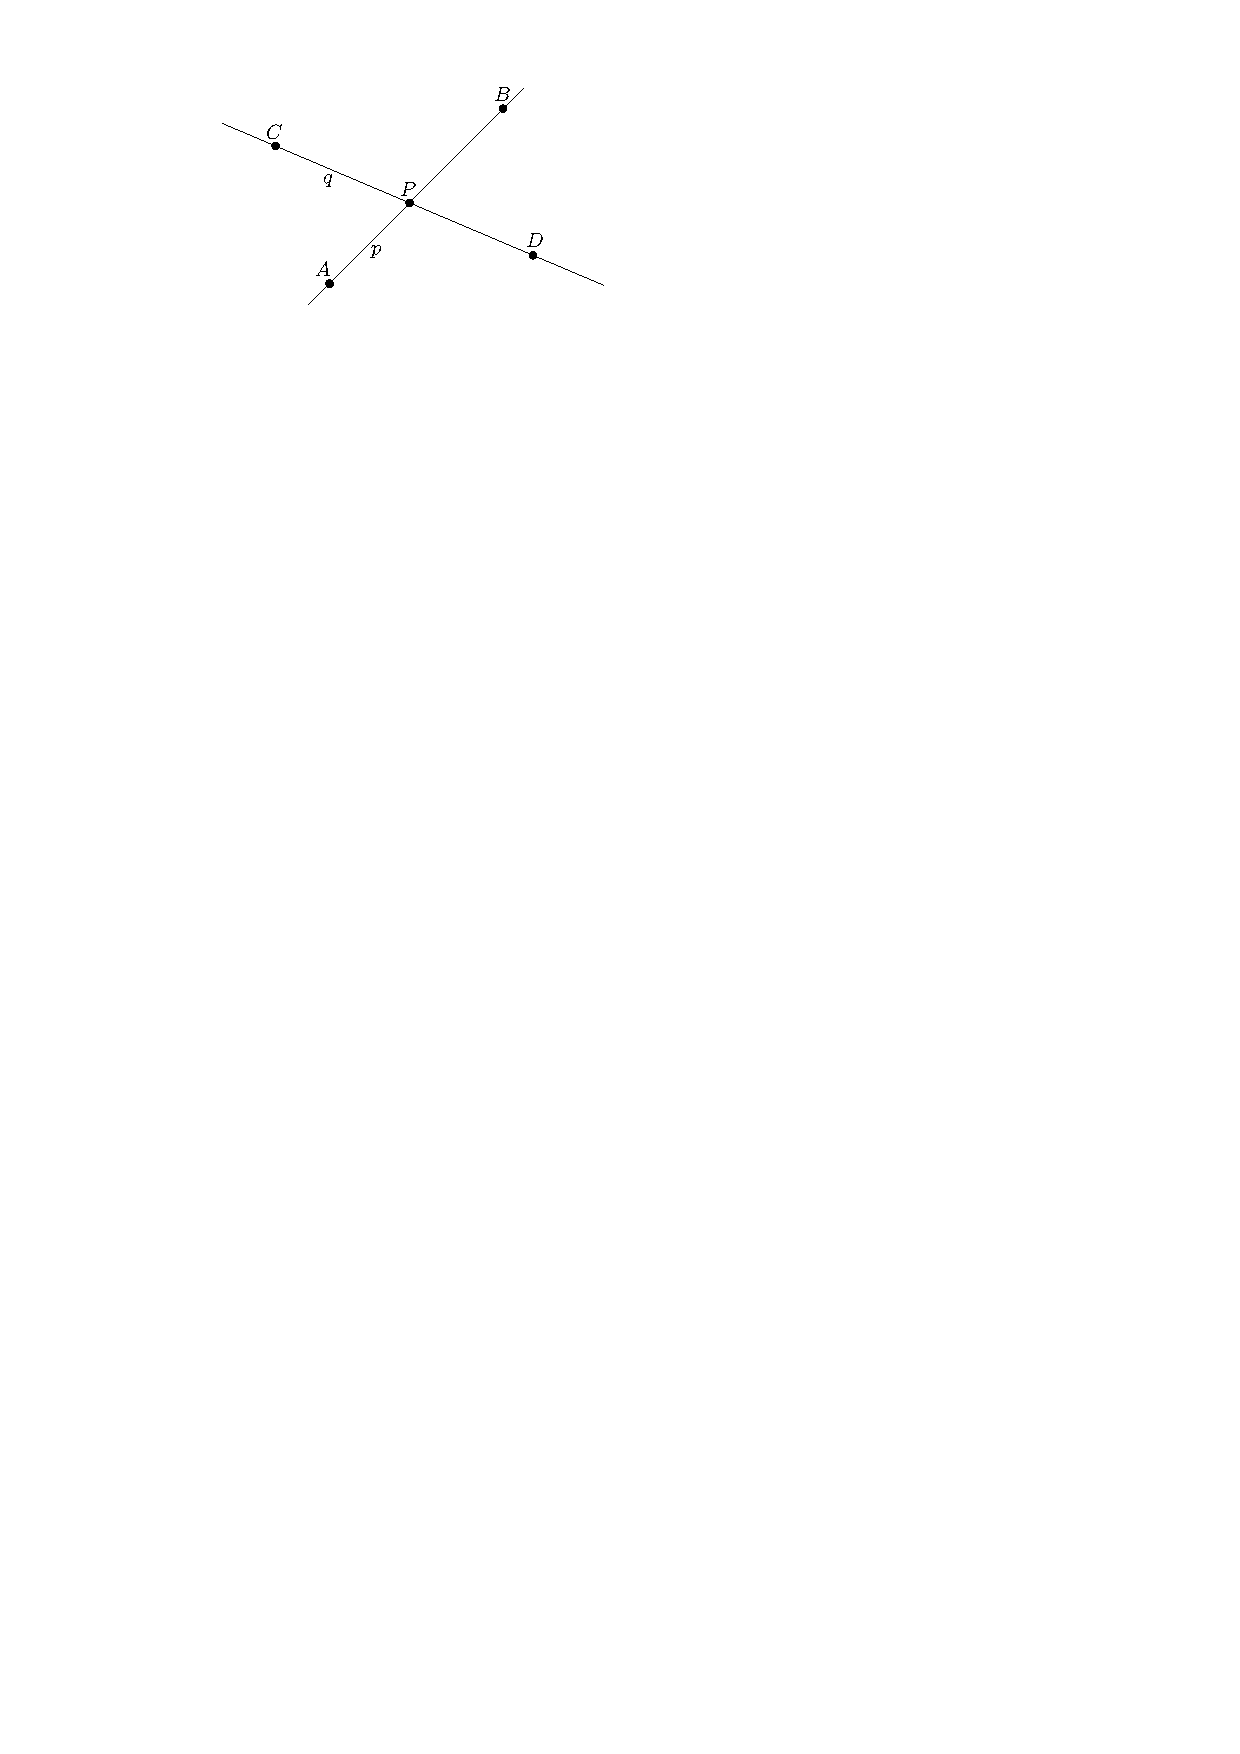
\includegraphics{../img/prusecik.pdf}
	\caption{Průsečík dvou přímek}
	\label{fig:prusecik}
\end{figure}

Průsečík musí ležet na obou přímkách a proto musí splňovat jejich obecné rovnice
$ax+by+c=0$.  Vyjádřeme si nyní obecné rovnice obou přímek. To můžeme
nejjednodušeji udělat pomocí normálových vektorů přímek. Mějme směrové vektory
přímek $p$: $u = (x_2-x_1,y_2-y_1)$ a $q$: $v=(x_4-x_3,y_4-y_3)$ pak normálové
vektory získáme jako $m = (-u_y,u_x)$ a $n = (-v_y,v_x)$. Obecná rovnice přímky
$p$ pak bude $m_xx+m_yy=c$ a přímky $q$ bude $n_xx+n_yy=d$. Koeficienty $c$ a
$d$ získáme dosazením bodů $A$ a $C$ do rovnic: $c = m_xx_1+m_yy_1$,
$d=n_xx_3+n_yy_3$. Pro průsečík musí platit obě rovnice, tedy 
\begin{eqnarray*}
m_xx+m_yy &=& m_xx_1+m_yy_1\\
n_xx+n_yy &=& n_xx_3+n_yy_3
\end{eqnarray*}
Tuto soustavu dvou rovnic o dvou neznámých můžeme řešit například pomocí
determinantů Cramerovým pravidlem $x_i = \frac{|A_i|}{|A|}$:

$$x = \frac{
	\begin{vmatrix}
		c & m_y \\
		d & n_y
	\end{vmatrix}
}
{
	\begin{vmatrix} 
		m_x & m_y \\
		n_x & n_y 
	\end{vmatrix}
}\,\!,\qquad
y = \frac{
	\begin{vmatrix}
		m_x & c \\
		n_x & d
	\end{vmatrix}
}
{
	\begin{vmatrix} 
		m_x & m_y \\
		n_x & n_y 
	\end{vmatrix}
}
$$

Pokud vzorec roznásobíme, získáme pro $x$-ovou souřadnici zlomek:
$$
x=\frac{(x_1 y_2-y_1 x_2)(x_3-x_4)-(x_1-x_2)(x_3 y_4-y_3 x_4)}
{(x_1-x_2)(y_3-y_4)-(y_1-y_2)(x_3-x_4)}$$
Tímto výrazem pak dokážeme jednoduše spočítat průsečík dvou přímek, pokud známe
souřadnice dvou bodů na každé z nich.

\section{Reprezentace čísel}
V~průběhu dalšího zpracování budeme potřebovat počítat průsečíky úseček daných
uzly. Protože průsečíky úseček nebudou mít celočíselné souřadnice, je potřeba
rozmyslet, jakým způsobem je reprezentovat.

{\tuc Čísla s~plovoucí desetinnou čárkou} se pro tyto účely nehodí, protože
nejsou přesná. Při výpočtech s~nimi vznikají zaokrouhlovací chyby, které mohou
zapříčinit špatné pořadí blízkých průsečíků v~uspořádání. Potřebujeme proto
přesnou reprezentaci.

{\tuc Zlomky} jsou pro reprezentaci desetinných čísel vhodnější. Dokážeme pomocí
nich přesně reprezentovat desetinná čísla. Zlomky můžeme vždy
upravit tak, aby jejich jmenovatel byl kladný.  Takové zlomky můžeme porovnávat
podle pravidla $\frac{a}{b} < \frac{c}{d} \Leftrightarrow a\cdot d < c\cdot b $. 
Pokud se nám ale stane, že porovnáváme dva zlomky, které mají vysoký čitatel i
jmenovatel, nemusí nám 64 bitů přesnosti stačit.

Předpokládejme, že máme město velikosti Prahy, což je přibližně $20 \times
30$\,km s~přesností na 10\,cm. O~úsečkách víme, že žádná nebude delší než 300
metrů, tudíž rozdíl jejich souřadnic nebude větší než 3\,000. Pokud budeme
maximalizovat jmenovatele, ze vzorce pro výpočet průsečíku vychází, že můžeme
dosáhnout nejvýše 9 milionů, protože jde o~součin dvou rozdílů souřadnic a každý
bude nejvýše 3\,000.

Tato situace opravdu může nastat, například pro vodorovnou a svislou úsečku
o~délce 300\,m, dotýkající se v~krajním bodě, tzn. $A=(3\,000,0),B=(0,0)$,
$C=(0,3000),D=(0,0)$. Tyto dvě mají průsečík, tudíž se nám mohou při počítání
vyskytnout. Pokud nyní vezmeme téměř totožnou situaci, ale úsečky budou posunuty
směrem k~maximu $x$-ové osy, pak bude $x$-ová souřadnice reprezentovat číslo
30\,km při přesnosti 10\,cm ve zlomku se jmenovatelem 9 milionů. Bude to tedy
číslo $30\cdot1\,000\cdot10\cdot9\cdot10^6=27 \cdot 10^{11}$. Na reprezentaci tohoto
čísla budeme potřebovat $\log_2 27\cdot 10^{11} \doteq 42$ bitů. Pokud tento
zlomek budeme chtít porovnat s~jiným zlomkem s~maximálním jmenovatelem, budeme
potřebovat $42 + \log_2 (9\cdot 10^{6}) \doteq 65$ bitů, na což nám 64bitová proměnná
nebude stačit.

{\tuc Smíšená čísla} nemají ani jednu z~předchozích nevýhod. Jsou to čísla,
která mají tvar $a+\frac{b}{c}$, kde $\frac{b}{c}<1$. Číslo $a$ nazvěme
základem, $b$ čitatelem a $c$ jmenovatelem. U~smíšených čísel je stejně jako
u~zlomků zachována přesnost, ale můžeme je porovnávat bez rizika přetečení.
Pokud se čísla liší v~základu, pak přeteční nehrozí, protože základy se
porovnávají přímo. Pokud mají dvě smíšená čísla stejné základy, pak porovnáme
jejich zlomky. To ale na rozdíl od přímého porovnávání zlomků není problém,
protože jmenovatel je opět nejvýše 24bitový a protože čitatel je nejvýše tak
velký jako jmenovatel, jejich vynásobením vznikne nejvýše 48bitové číslo.
Protože proměnné máme 64bitové, nikde k~přetečení nedojde.

Smíšená čísla jsou implementována jako struktury se členy \verb|base| pro
základ, \verb|numer| pro čitatele a \verb|denom| pro jmenovatele. Všechny
položky jsou 64bitová celá čísla a jmenovatel nesmí být záporný. Pro práci se
smíšenými čísly jsou definovány pomocné funkce v~souboru \verb|mixnum.h|.

\section{Spojky mezi cestami}
\subsection{Příprava dat}
Spojky budeme vytvářet mezi cestami, po kterých budeme posléze vyhledávat.
Nejprve si proto všechny cesty ve funkci \verb|makeGraph| projdeme a roztřídíme
do dvou polí. 

Pole \verb|wayGraph| obsahuje pro každý uzel pole všech jeho sousedů po cestách,
po kterých se bude vyhledávat. Pole \verb|barGraph| obsahuje ty dvojice indexů
uzlů, které spolu sousedí na některé cestě označené jako překážka. Obě pole
reprezentují graf, první pomocí seznamu sousedů, druhé pomocí seznamu hran.
Každé pole budeme využívat jiným způsobem, a proto se nám hodí různá
reprezentace.

Jako druhý krok nalezneme všechny kandidáty na spojky. Zde využijeme mřížky.
Protože spojky chceme dlouhé nejvíce 20 metrů a mřížka má čtverce o~hraně také
20 metrů, stačí nám při hledání možných spojek pro daný bod se podívat pouze na
body ve čtverci, kde sám leží, v~sousedních čtvercích napravo od něj (nahoře,
uprostřed a dole) a ve čtverci pod ním. Protože jsou spojky kratší než 20\,m,
nemohou dále než do sousedního čtverce dosáhnout a protože procházíme postupně
všechny čtverce, možné spojky doleva a nahoru již známe ze zpracování
předchozích čtverců. 

Jednotlivé počáteční a koncové body spojek získáme ze všech bodů v~daném čtverci
vytříděním těch, které mají nějaké sousedy v~poli \verb|wayGraph|. Nepřidáváme
ale všechny spojky, protože pak existovalo např. u kruhových cest v parcích
mnoho spojek, které nepřinášely výrazné zlepšení. Zvolili jsme proto náhodný
výběr, při němž pro každý bod vybereme z každého čtverce mřížky jen několik
kandidátů. Zkoumali jsme vliv počtu kandidátů na délku trasy a jako optitmum se
ukázalo zvolit dva body jako kandidáty z každého čtverce mřížky. Při větším
množství bodů se výslledky zlepšovaly přibližně o procento, ale velikost
výstupního souboru rostla přibližně o šest procent.

%TODO: obrázek

\subsection{Datové struktury}
Když máme připravené kandidáty na spojky a seznam všech překážek, můžeme
přistoupit k~zametání roviny. Zametání roviny probíhá ve funkci
\verb|findDirectWays|. Nejprve popíšeme používané struktury a proměnné.

Struktura \verb|line_t| reprezentuje úsečku v~rovině. Při vytváření se jí
nastavují tyto atributy:
\begin{itemize}
	\item \verb|startlon| a \verb|startlat| udávají souřadnice začátku
	úsečky. Začátek úsečky má vždy nejvýš tak velkou souřadnici $x$, jako
	konec.
	\item \verb|endlon| a \verb|endlat| udávají souřadnice konce úsečky.
	Souřadnice začátků a konců jsou vždy celočíselné, proto je
	reprezentujeme 64bitovými celými čísly.
	\item \verb|startid| a \verb|endid| udávají identifikátor začátku a
	konce úsečky v~OSM.
	\item \verb|isBar| říká, jestli je daná úsečka překážkou.
\end{itemize}
V~průběhu zametání roviny jsou úsečkám nastavovány následující atributy:
\begin{itemize}
	\item \verb|broken| říká, jestli má průsečík s~jinou úsečkou a alespoň
	jedna z~nich je překážka.
	\item \verb|started| udává, že byla zařazena do průřezu.
	\item \verb|ended| udává, že byla v~průžezu a již skončila.
\end{itemize}

Globální pole \verb|lines| s prvky typu \verb|line_t| obsahuje všechny kandidáty
na spojky, globální pole \verb|bars| s prvky typu \verb|line_t| obsahuje všechny
překážky. 

Pro zametání budeme také potřebovat haldu, ze které budeme vybírat nejbližší
událost. V~našem případě používáme haldy dvě, první (\verb|seQueue|), kterou na
začátku naplníme událostmi začátek a konec úsečky, a druhou (\verb|intQueue|),
kterou budeme průběžně plnit průsečíkovými událostmi. V~každém průběhu hlavního
cyklu pak vybereme tu událost, která nastane dříve. Samotné haldy jsou pak
reprezentovány v~poli pomocí binárních hald z~LibUCW. 

Haldy obsahují struktury typu \verb|event_t| respektive \verb|int_event_t| pro
počáteční a koncové respektive průsečíkové události. Struktury mají následující
prvky:
\begin{itemize}
	\item \verb|lon| a \verb|lat| udávají souřadnice události. V~případě
	začátků a konců se jedná o~64bitová celá čísla, v~případě průsečíků se
	jedná o~čísla smíšená. 
	\item \verb|dlon| a \verb|dlat| udávají směrnici úsečky, které se
	událost týká. V~případě průsečíků se jedná o~tu, která by byla
	zpracována dříve.
	\item \verb|lineIdx| je index úsečky, které se událost týká
	\item \verb|line2Idx| se vyskytuje pouze u~průsečíků a jde o~index druhé
	úsečky, které se událost týká.
\end{itemize}


\subsection{Reprezentace průřezu}
Také budeme potřebovat vyhledávací strom, ve kterém si budeme pamatovat aktuální
pořadí úseček v~průřezu. Pro jeho reprezentaci jsme zvolili červeno-černé stromy
z~LibUCW. V~jeho vrcholech jsou uloženy jednotlivé úsečky, které jsou aktuální
pro daný průřez. Protože se ale úsečky mohou křížit, použili jsme několik
vlastních rozšíření. 

Museli jsme si napsat vlastní {\tuc porovnávací funkci}. Zametáme podle $x$-ové
souřadnice tudíž ve stromě potřebujeme mít úsečky seřazené podle $y$-ové
souřadnice v~daném bodě. Ta se ale s~kažým posunutím zametací přímky mění,
proto ve stromě najdeme pouze indexy do pole \verb|lines| na jednotlivé úsečky.
Porovnávací funkce dostane tyto indexy, z~globální proměnné \verb|lon| zjistí,
jaká je aktuální $x$-ová souřadnice zametací přímky, a vypočítá $y$-ovou
souřadnici porovnávaných úseček v~daném bodě. Pokud se $y$-ové souřadnice liší,
pak vrátí výsledek, pokud jsou shodné, porovnávají se podle úhlu. 

K~tomuto je zapotřebí globální proměnná \verb|anglesign|, která říká, s~jakým
znaménkem se má úhel brát. Pokud totiž srovnáváme úsečky při přidávání, zajímá
nás, v~jakém úhlu pokračují dále, naopak při odebírání nás zajímá, pod jakým
úhlem přicházejí. Seřazení je v~tomto případě přesně opačné. Úsečka, která
mířila nejvíce k~severu, tudíž byla na začátku poslední z~daného bodu, bude na
konci přicházet z~jihu, tudíž bude mezi prvními. Úhly úseček nepotřebujeme
počítat, stačí nám porovnat jejich směrnice, což jsou zlomky, a to umíme rychle
a beze ztráty přesnosti.

Ve stromě dále musíme umět prohodit dva sousední vrcholy při průsečíku jim
odpovídajících úseček. Protože si ve vrcholech pamatujeme pouze indexy do pole
úseček, stačí při překřížení tyto indexy prohodit. Struktura stromu i korektnost
uspořádání tím zůstanou zachovány.

Stromy v~LibUCW umí i mazání vrcholu podle pointeru na něj, což se nám hodí při
událostech konec úsečky, protože ji nemusíme hledat, ale stačí si při vytváření
úsečky uložit pointer na vrchol stromu do pole \verb|lineNodes| a při křížení
úseček prohodit patřičné ukazatele. Při mazání se pak jen podíváme podle indexu
úsečky do správného místa v~poli a patřičný vrchol smažeme. Je to výhodou i
v~situaci, kdy nastal při zametání nějaký problém a neproběhla nějaká událost
křížení, a tudíž bychom standardní cestou vrchol nenašli.

Při vkládání nového vrcholu do stromu také potřebujeme zjistit sousedy nově
vloženého vrcholu, abychom přidali případné události křížení. Tuto funkci stromy
v~LibUCW již také obsahují, tudíž nám stačí ji jen využít. Sousedy rovněž
hledáme při křížení, protože překřížením úseček se sousedství změnilo.


\subsection{Zametání}
Události procházíme seřazené nejprve podle délky, pak podle šířky. Pokud jsou
dvě události na stejném místě, nejprve se zpracují události konce úsečky, poté
průsečíky a nakonec události začátku úsečky. Pokud nastane více událostí téhož
typu na stejném místě, zpracovávají se podle úhlu úseček, viz rozbor pořadí ve stromě. 

Dokud máme v~haldě nějaké události, vybereme vždy tu nejbližší a zpracujeme ji.
Pokud se jedná o~začátek úsečky, zkontrolujeme, jestli ve stromě již není, či
zda v~něm není nějaká, se kterou by byla nerozlišitelná. Protože dvě úsečky,
které leží přesně přes sebe jsou nedefinovaný stav, tak tu, která přijde ke
zpracování jako druhá, ignorujeme. Úsečku následně vložíme do průřezového stromu
a zkontrolujeme sousední úsečky, zda se s~nově přidanou nekříží. Pokud ano, tak
přidáme příslušné průsečíkové události do průsečíkové haldy.

Jedná-li se o~konec úsečky, zkontrolujeme, zda úsečka začala (byla přidána do
stromu). Pokud ne, skončíme. Následně zjistíme, zda odstraněním této úsečky se
její sousedé neprotnou, případně přidáme průsečíkovou událost. Nakonec úsečku
smažeme z~průřezového stromu.

Pokud se jedná o~průsečík, nejprve zkontrolujeme, jestli jsme danou událost již
nezpracovali. Pokud se totiž dvě úsečky protínají a během toho, co se k~sobě
přibližují se mezi nimi objeví další úsečka, vznikne průsečíková událost těchto
dvou krajních přímek poprvé při přidání pozdější z~nich a podruhé při konci
vnitřní úsečky, přitom se stále jedná o~stejný průsečík. Protože tyto dvě
průsečíkové události se seřadí hned za sebe a protože se každé dvě úsečky
protnou nejvýše jednou, stačí nám si pamatovat poslední událost a pokud je nová
průsečíková událost se stejnými úsečkami, můžeme ji zahodit.

Dále zkontrolujeme, jestli některá z~úseček již neskončila. Pokud se dvě úsečky
potkávají v~koncovém bodě, pak je zbytečné řešit jejich průsečík. Proto nejprve
vyřešíme konce úseček a pokud máme řešit průsečík s~již skončenou úsečkou,
můžeme ho ignorovat. Následně zjistíme, která z~úseček je nyní horní a která
dolní, a prohodíme odkazy na vrcholy stromu v~poli \verb|lineNodes| a rovněž
prohodíme indexy úseček ve vrcholech stromu. Nakonec zjistíme, zda po prohození
nevznikly nové průsečíky, a případně přidáme průsečíkové události.

Když celý cyklus doběhne, přidáme funkcí \verb|addDirectToMap| do seznamu cest
nově vzniklé spojky a jsme hotovi.


\section{Zkratky přes průchozí prostranství}
Abychom mohli vytvářet zkratky přes průchozí prostranství, potřebujeme nejprve
zjistit, které všechny uzly se vyskytují v~tomto prostranství. Pro samotné
vytváření zkratek pak použijeme obdobný způsob jako při hledání spojek mezi
cestami. 

Nejprve vytvoříme pole všech průchozích prostranství.  K~tomuto účelu
slouží funkce \verb|findWalkAreas|. Procházíme postupně všechny cesty a u~každé
kontrolujeme, jestli se jedná o~průchozí prostranství. Pokud ano, pak vytvoříme
strukturu \verb|walk_area_t| obsahující data o~této ploše: Zjistíme, do jakého
podobélníku mřížky plocha zasahuje, a z~tohoto podobdélníku vybereme ty body,
které jsou uvnitř plochy. Body přidáme do pole \verb|nodeIdxs| a cesty do pole
\verb|ways|. Cesty potom rozdělíme na překážky, jejichž indexy uložíme do
atributu \verb|barIdxs| a vyhledávatelné cesty, které uložíme do atributu
\verb|wayIdxs|. Během rozdělování také odstraňujeme duplicitní cesty. 

Jako další krok připravíme kandidáty na zkratky. Použijeme k tomu funkci
\verb|makeAreaCandidates|. Procházíme postupně dvojice bodů v~dané ploše a
hledáme bližší než 300\,m, které nejsou na společné cestě. Neuvažujeme ovšem
všechny dvojice, ale vybíráme pro každý uzel náhodně z ostatních uzlů, protože
při uvažování všech dvojic vznikalo mnoho cest v podobných místech podobným
směrem. Nalezené dvojice následně přidáme do seznamu kandidátů. Experimentálně
jsme zkoumali vliv průměrného počtu sousedů pro jeden vrchol na délku nalezených
cest přes pražskou Stromovku a Letnou. Jako optimální se ukázalo vybírat pro
každý vrchol průměrně dva sousedy. K dalšímu výrazném zlepšení totiž došlo až
pro pět sousedů, což ale při zlepšení o přibližně 10 procent vedlo ke zvýšení
velikosti grafu o 20 procent, což nám již  přišlo nevýhodné.

Vytvoříme také seznam překážek funkcí \verb|makeAreaBarGraph|. Nejprve přidáme
všechny překážky ze seznamu \verb|barIdxs|, poté přidáme všechny cesty
z~\verb|wayIdxs| a nakonec přidáme obvod plochy. Cesty přidáváme proto, aby
nevnikalo příliš mnoho zkratek, což by vedlo ke zvětšování vyhledávacího grafu.
Takto vzniknou pouz zkratky přes volná prostranství a nebudou křížit cesty.

Když máme kandidáty na zkratky i seznam překážek, můžeme použít již popsané funkce
\verb|findDirectWays| a \verb|addDirectToMap| k~odstranění kandidátů
kolidujících
s~překážkami a cestami a k~přidání výsledných zkratek do mapy. Postup od přípravy
kandidátů až po jejich přidání do mapy zopakujeme pro každou průchozí plochu.

\section{Vytvoření vyhledávacího grafu}
Když již máme všechna data připravená, vytvoříme vyhledávací graf. Nejprve do
něj přidáme všechny vrcholy a hrany. Následně graf projdeme do hloubky a
vybereme tu komponentu, která je největší. Poté v~grafu necháme jen vrcholy a
hrany, které do této komponenty patří, a graf uložíme do souboru
\verb|praha-graph.pbf|. 

\chapter{Hledání tras}
Součástí naší práce bylo i vytvoření jednoduchého vyhledávače nad připravenými
daty. Vyhledávač má textový i grafický režim a cestu hledá Dijkstrovým
algoritmem. Rychlosti přesunu po jednotlivých kategoriích hran (viz str.
\pageref{label:kategorie}) můžeme nastavit pomocí konfiguračního souboru.
Program také umožňuje uložit nalezenou trasu jako soubor GPX. \cite{gpxspec}  

\section{Konfigurace}
Vyhledávač umožňuje konfigurovat rychlosti pohybů po hranách jednotlivých
kategorií dvěma způsoby. První je zadáním absolutní rychlosti a druhý je zadáním
poměru k~rychlosti pohybu po obecné cestě. Také je možné konfigurovat penalizaci
za převýšení.

Konfigurační soubor \verb|speeds.yaml| je ve formátu YAML: \cite{yamlspec} 
\begin{verbatim}
speeds:
        WAY: 6
        PARK: 4
        GREEN: 3
ratios:
        PAVED: 1.2
        STEPS: 0.6
heights:
        upscale: 1
        downscale: 1
\end{verbatim}
Konfigurační soubor obsahuje mapu se třemi klíči:
\begin{itemize}
	\item Klíč \verb|speeds| slouží k~nastavení absolutních rychlostí pohybu
	pro jednotlivé kategorie hran. Obsahuje jako hodnotu mapu, jejímiž klíči jsou
	názvy kategorií a hodnotami rychlosti pohybu po cestách dané kategorie
v~kilometrech za hodinu. Vždy je potřeba nastavit rychlost pro kategorii
	\verb|WAY|, z~ní se počítají poměrné rychlosti.
	\item Klíč \verb|ratios| slouží k~nastavení poměrných rychlostí vzhledem
	k~rychlosti kategorie \verb|WAY|. Jeho hodnotou je stejná mapa jako
u~klíče \verb|speeds|, ale jako hodnoty se udávají poměry k~rychlosti
	kategorie \verb|WAY|. Pokud se nějaká kategorie vyskytne v~mapách pro
	oba klíče \verb|speeds| a \verb|ratios|, má prioritu absolutní rychlost
	z~klíče \verb|speeds|.
	\item Klíč \verb|heights| umožňuje nastavit penalizaci za převýšení.
	Jako hodnotu obsahuje mapu s~klíči \verb|upscale| a \verb|downscale|,
	které udávají, za kolik vodorovných metrů se bude počítat jeden metr
	převýšení při chůzi směrem do kopce a z~kopce. Je možné nastavit kladné,
	záporné hodnoty i nulu, při které se bude převýšení ignorovat. Pokud by
	měla cesta mít po započítání převýšení zápornou délku, je délka
	považována za nulovou.
\end{itemize}

\section{Dijkstrův algoritmus}
Dijkstrův algoritmus \cite{dijkstra} slouží k~nalezení nejkratší cesty mezi dvěma vrcholy grafu.
Algoritmus postupně prohledává graf a zpracovává vrcholy. Vrcholy mohou mít tři
stavy: nedosažený, otevřený a zpracovaný. U~každého vrcholu $v$ také udržujeme
nejkratší dosud známou vzdálenost $d(v)$ z~výchozího vrcholu do daného vrcholu. 
Během procházení grafu si udržujeme množinu otevřených vrcholů. Délku hrany
$(u,v)$ budeme označovat $l(u,v)$.

Na začátku jsou všechny vrcholy nedosažené a jejich vzdálenost je nekonečno.
Označíme výchozí vrchol jako otevřený a přidáme ho do množiny. Jeho vzdálenost
změníme na nulu a opakujeme následující postup:
\begin{enumerate}
	\item Odebereme z~množiny vrchol $v$ s~nejmenší vzdáleností. 
	\item Pokud je $v$ vrchol cílový, našli jsme nejkratší cestu a končíme.
	\item Všem jeho nedosaženým sousedům $u$ nastavíme $d(u)=d(v)+l(v,u)$,
	označíme je jako otevřené a přidáme je do množiny oteřených vrcholů.
	\item Pokud pro nějakého otevřeného souseda $u$ platí $d(u) >
	d(v)+l(u,v)$, pak upravíme $d(u)$ na $d(v)+l(v,u)$.
	\item Vrchol $v$ označíme za zpracovaný.
\end{enumerate}
Pro reprezentaci množiny otevřených vrcholů můžeme výhodně použít haldu, protože
do množiny pouze přidáváme prvky, snižujeme jejich hodnotu a odebíráme z~něj
minimum.

Bylo by možné použít i jiné algoritmy pro hledání nejkratší cesty
\cite{dijkstra}, například A*,  ale Dijkstrův
algortmus je pro hledání ve městě velikosti Prahy dostatečně rychlý a je možno
jej bez problémů použít.


\section{Implementace}
Výkonný kód je uložen v~souboru \verb|searchlib.c|. Jak textový vyhledávač
\verb|search|, tak grafický vyhledávač \verb|QOsmWalk| jsou pouze nadstavby
volající funkce definované v~\verb|searchlib.c|. Program vyžaduje knihovny {\tuc libyaml} a
{\tuc PROJ.4}. Program také používá makra z~{\tuc LibUCW}, ale nepotřebuje být s~touto
knihovnou slinkován. Grafická nadstavba \verb|QOsmWalk| je napsána v~prostředí
Qt.

Soubor \verb|searchlib.c| poskytuje dvě funkce, které pokrývají plně potřeby
vyhledávače. První z~nich je funkce \verb|prepareData|, která načte vyhledávací
graf a konfigurační soubor s~rychlostmi, načež připraví data pro konverzi WGS-84
$\leftrightarrow$ UTM, vytvoří pole \verb|nodeWays|, které pro každý vrchol
obsahuje seznam hran s~ním incidentních a spočítá a uloží délky všech hran. Tuto
funkci stačí zavolat jen jednou při startu programu a uložit si strukturu
s~připravenými daty pro hledání, kterou vrátí.

Druhou z~funkcí je \verb|findPath|, která slouží k~opakovanému hledání pěších
tras. Tato funkce dostane data připravená první funkcí a dvojici zeměpisných
souřadnic. Najde cestu mezi vrcholem v~grafu nejblíže prvním souřadnicím a
vrcholem v~grafu nejblíže druhým souřadnicím. Funkce vrátí strukturu typu
\verb|search_result_t|, která obsahuje pole vrcholů popisující trasu a údaje o~délce
trasy.

Při hledání trasy nejprve převedeme zadané zeměpisné souřadnice do formátu UTM,
ve kterém jsou uloženy souřadnice bodů v~grafu, a následně najdeme nejbližší
vrchol k~zadaným souřadnicím. Poté si připravíme struktury pro Dijkstův
algoritmus a pomocí něj najdeme nejkratší trasu. Nakonec projdeme grafem po
zpětných hranách, vytvoříme pole obsahující procházené body trasy a vrátíme
výsledek.

Abychom mohli spustit Dijkstrův algoritmus, potřebujeme si pro každý vrchol
pamatovat pomocná data. Tato data nemáme uložena přímo v~grafu, ale v~poli
\verb|dijArray|, které má za položky struktury typu \verb|dijnode_t|. Tyto
struktury obsahují následující položky:
\begin{itemize}
	\item \verb|fromIdx| -- ze kterého vrcholu jsme přišli 
	\item \verb|fromEdgeIdx| -- po které hraně jsme přišli
	\item \verb|reached| -- bylo už vrcholu dosaženo? 
	\item \verb|completed| -- byl už vrchol zpracován?
	\item \verb|dist| -- délka nejkratší známé cesty do daného vrcholu
\end{itemize}

Při každé
změně vzdálenosti do nějakého vrcholu si uložíme, z~jakého vrcholu jsme do něj
přišli a po které hraně. Díky tomu pak můžeme projít zpět po těchto uložených
hranách a získáme tím i vrcholy nejkratší cesty. Naší drobnou úpravou je obrácení směru
hledání od cílového vrcholu k~výchozímu. Potom je průchod po zpětných hranách
přímo průchod nejkratší cestou od výchozího bodu k~cílovému. Protože ale
používáme i výšky jednotlivých vrcholů, nejsou hrany v~obou směrech stejně
ohodnocené a proto při hledání od cíle k~výchozímu vrcholu musíme počítat
s~výškami, jako bychom šli v~opačném směru, než jak vede hrana.

Když je cesta nalezena, jen projdeme po zpětných hranách a uložíme nalezenou
cestu do pole. Běhm procházení nalezené cesty převádíme souřadnice vrcholů zpět
z~UTM do WGS-84 a v~této soustavě je také ukládáme v~poli. Každý vrchol má také
uložen v~prvku \verb|type| kategorii hrany, po níž přechází do následujícího
vrcholu. Poslední vrchol má kategorii nastavenu na $-1$.

\chapter{Experimenty}
Po dokončení jsme náš vyhledávač OsmWalk vyzkoušeli na hledání pěších tras po
Praze. Zkoumali jsme rychlost vyhledávání tras, jejich vhodnost a správnost
odhadu času a vzdálenosti. Také jsme udělali několik měření porovnávající různé
dostupné vyhledávače cest.

Každá porovnávaná trasa obsahuje popis, obrázek ukazující nalezené cesty
jednotlivých vyhledávačů a srovnání parametrů nalezených cest. Položka {\it
Vlastní měření} je naměřený čas a vzdálenost při chůzi po trase nalezené naším
vyhledávačem. 

\section{Trasa středem města}
Trasa vedoucí od Čertovky na Florenc. Trasa prochází středem města, což je hustá
zástavba bez větších volných ploch. Většina území je pěší zóna, tudíž nejsou
problémy se špatnou návazností chodníků v mapových podkladech. Vylepšení našeho
vyhledávače v podobě spojek ani zkratek by zde nemělo hrát velkou roli.
\begin{itemize}
	\item OsmWalk: 2.5\,km, 25\,min
	\item Mapy.cz: 2.7\,km, 40\,min
	\item Google maps: 2.5\,km, 31\,min
	\item OsmAnd: 2.6\,km, 30\,min
	\item Vlastní měření: 2.5\,km, 26\,min
\end{itemize}
Nalezené trasy byly přibližně stejně dlouhé a kromě Map.cz se lišily jen
minimálně. Čas Map.cz se s holedem na délku jevil jako přemrštěný, odhad délky a
času našeho vyhledávače byl přesný. 


\section{Trasa přes most Barikádníků}
Trasa vedoucí z kolejí 17.~listopadu na autobusovou zastávku Nádraží Holešovice.
Na této trase je podstatné, že hledáme trasu pro pěší a nechceme chodit po
šestiproudé magistrále. Optimální cesta používaná studenty kolejí obsahuje
několik pěšin, které nemusí být dobře zmapovány, tudíž zde je možnost využití
spojek a zkratek.

\begin{figure}[h]
	\centering
	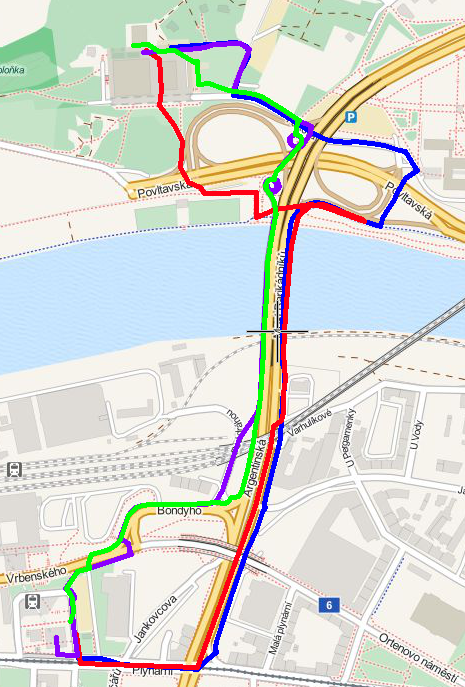
\includegraphics[width=12cm]{../img/kol-hol.png}
	\caption{Trasa přes most Barikádníků}
	\label{fig:kol-hol}
\end{figure}

\begin{itemize}
	\item OsmWalk: 1.3\,km, 14\,min
	\item Mapy.cz: 1.7\,km, 26\,min
	\item Google maps: 1.6\,km, 22\,min
	\item OsmAnd: 1.6\,km, 21\,min
	\item Vlastní měření:
\end{itemize}
Trasy nalezené jednotlivými vyhledávači se zde výrazně lišily. Podrobnější
zkoumání ukázalo, že ani Mapy.cz ani Google Maps neumí správně používat podchod
pod ulicí Povltavská. Tyto vyhledávače také přešly z chodníku na silnici,
Mapy.cz v místě, kdy už po obou stranách silnice vede chodník, Google Maps už
dříve, v místě, kde vede chodník odděleně od silnice. Naproti tomu OsmAnd našel
trasu zcela korektně po chodnících a uměl i správně použít podchod. Náš
vyhledávač našel téměř optimální trasu, problém mu dělaly rampy z podchodu na
most. Na konci naplánoval trasu po spojce mimo přechod, což ale není vadou.
%TODO Ověření odhadu.

\section{Trasa přes Petřín}
Trasa vedoucí z Malostranského náměstí na koleje Strahov. Převážná část této
trasy vede přes petřínský park, tudíž je zde potenciál pro využití zkratek. 

\begin{figure}[h]
	\centering
	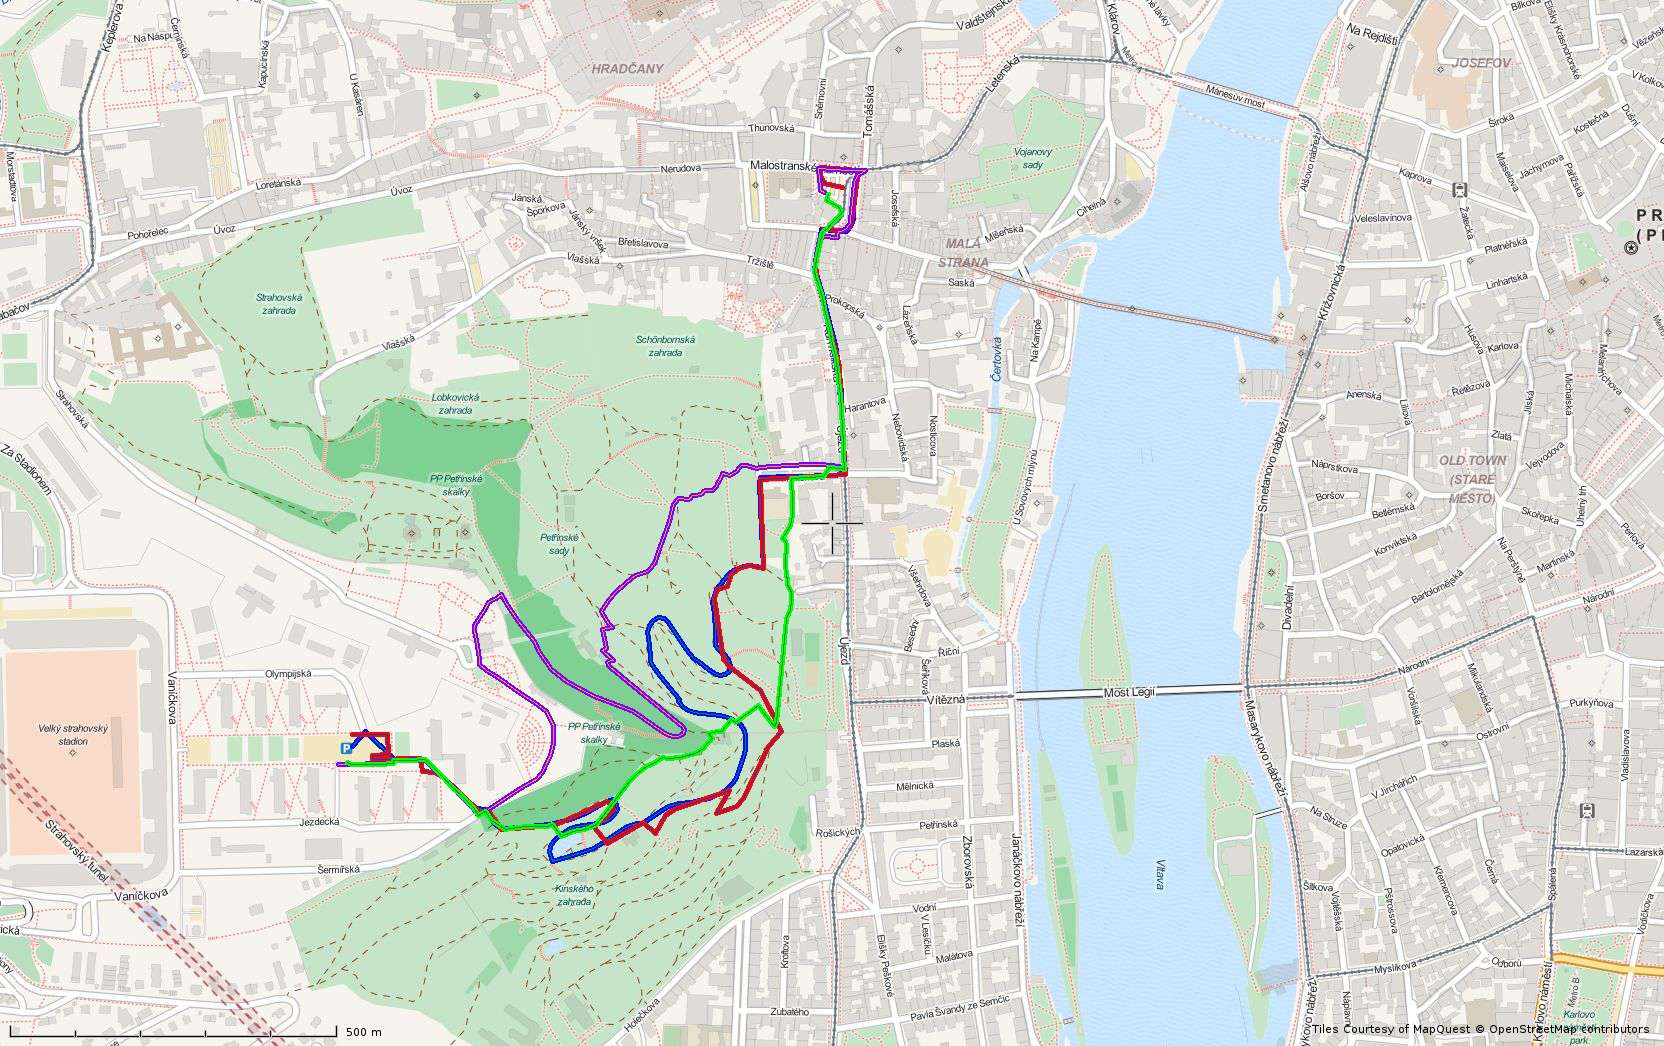
\includegraphics[width=12cm]{../img/ms-sh.png}
	\caption{Trasa přes Pteřín}
	\label{fig:kol-hol}
\end{figure}
\begin{itemize}
	\item OsmWalk: 1.7\,km, 25\,min
	\item Mapy.cz: 2.4\,km, 36\,min
	\item Google maps: 2.2\,km, 33\,min
	\item OsmAnd: 2.4\,km, 28\,min
	\item Vlastní měření: 1.8\,km, 21\,min
\end{itemize}


% Ukázka použití některých konstrukcí LateXu (odkomentujte, chcete-li)
% \include{ukazka}

\chapter*{Závěr}
\addcontentsline{toc}{chapter}{Závěr}

zrychleni - potencialova heuristika, viz MJ - skripta z GA

skriptovani vypoctu penalt

Další možné rozšíření systému penalt by mohlo být například posuzování intervalů
linek, kdy bychom mohli preferovat častěji jedoucí linky. 

posun odchodu podle prvniho MHD

okolí cest


%%% Seznam použité literatury
\def\bibname{Seznam použité literatury}
%%% Seznam použité literatury je zpracován podle platných standardů. Povinnou citační
%%% normou pro bakalářskou práci je ISO 690. Jména časopisů lze uvádět zkráceně, ale jen
%%% v kodifikované podobě. Všechny použité zdroje a prameny musí být řádně citovány.

\def\bibname{Seznam použité literatury}
\begin{thebibliography}{99}
\addcontentsline{toc}{chapter}{\bibname}

\bibitem{lamport94}
  {\sc Lamport,} Leslie.
  \emph{\LaTeX: A~Document Preparation System}.
  2. vydání.
  Massachusetts: Addison Wesley, 1994.
  ISBN 0-201-52983-1.

\bibitem{osmweb}
	\emph{OpenStreetMap} [online]. 
	2014, 4.5.2014 [cit. 2014-05-04]. 
	Dostupné z: \url{http://www.openstreetmap.org}

\bibitem{osmxml}
	\emph{OSM XML} [online]. 
	2014, 16 September 2013 [cit. 2014-05-06]. 
	Dostupné z: \url{http://wiki.openstreetmap.org/wiki/OSM_XML}

\bibitem{osmfeatures}
	\emph{Cs: Map Features} [online]. 
	2014-04-01 [cit. 2014-05-17]. 
	Dostupné z: \url{http://wiki.openstreetmap.org/wiki/Cs:Map_Features}

\bibitem{wgsnorma}
	{\sc NIMA.}
	\emph{World geodetic system 1984} [online]. 
	3. vydání, 1. dodatek.
	3 January 2000 [cit. 2014-05-04]. 
	Dostupné z: \url{http://www2.jpl.nasa.gov/srtm/}.

\bibitem{utmnorma}
	{\sc Snyder,} John P.
	\emph{Map Projections: A~Working Manual} [online]. 
	1987, [cit. 2014-05-08]. 
	Dostupné z: \url{http://pubs.er.usgs.gov/publication/pp1395}.

\bibitem{srtmweb}
	{\sc NASA.}
	\emph{The Shuttle Radar Topography Mission} [online]. 
	2014, June 17, 2009 [cit. 2014-05-04]. 
	Dostupné z: \url{http://www2.jpl.nasa.gov/srtm/}.

\bibitem{pbfweb}
	{\sc Google.}
	\emph{Protocol Buffers} [online]. 
	2014, April 2, 2012 [cit. 2014-05-05]. 
	Dostupné z: \url{https://developers.google.com/protocol-buffers/}.

\bibitem{pbfenc}
	{\sc Google.}
	\emph{Encoding - Protocol Buffers} [online]. 
	2014, April 2, 2012 [cit. 2014-05-07]. 
	Dostupné z: \url{https://developers.google.com/protocol-buffers/docs/encoding}.

\bibitem{pbfspec}
	{\sc Google.}
	\emph{Language Guide - Protocol Buffers} [online]. 
	2014, April 22, 2014 [cit. 2014-05-07]. 
	Dostupné z:	\url{https://developers.google.com/protocol-buffers/docs/proto}.

\bibitem{lineint}
	{\sc Weisstein} Eric W.
	\emph{Line-Line Intersection.} [online]. 
	2014, May 12, 2014 [cit. 2014-05-12]. 
	Dostupné z:	\url{http://mathworld.wolfram.com/Line-LineIntersection.html}.

\bibitem{zametani}
	{\sc Mareš} Martin
	\emph{Geometrické algortimy} [online]. 
	2014, 17.11.2013 [cit. 2014-05-13]. 
	Dostupné z:	\url{http://mj.ucw.cz/vyuka/ads/43-geom.pdf}.
	

\end{thebibliography}



%%% Tabulky v bakalářské práci, existují-li.
%\chapwithtoc{Seznam tabulek}

%%% Použité zkratky v bakalářské práci, existují-li, včetně jejich vysvětlení.
%\chapwithtoc{Seznam použitých zkratek}

%%% Přílohy k bakalářské práci, existují-li (různé dodatky jako výpisy programů,
%%% diagramy apod.). Každá příloha musí být alespoň jednou odkazována z vlastního
%%% textu práce. Přílohy se číslují.
\chapwithtoc{Přílohy}

\openright
\end{document}
